
%%%%%%%%%%%%%%%%%%%%%%% file typeinst.tex %%%%%%%%%%%%%%%%%%%%%%%%%
%
% This is the LaTeX source for the instructions to authors using
% the LaTeX document class 'llncs.cls' for contributions to
% the Lecture Notes in Computer Sciences series.
% http://www.springer.com/lncs       Springer Heidelberg 2006/05/04
%
% It may be used as a template for your own input - copy it
% to a new file with a new name and use it as the basis
% for your article.
%
% NB: the document class 'llncs' has its own and detailed documentation, see
% ftp://ftp.springer.de/data/pubftp/pub/tex/latex/llncs/latex2e/llncsdoc.pdf
%
%%%%%%%%%%%%%%%%%%%%%%%%%%%%%%%%%%%%%%%%%%%%%%%%%%%%%%%%%%%%%%%%%%%


\documentclass[runningheads,a4paper]{llncs}
\usepackage{graphicx}
\usepackage{url}
\usepackage[listings]{tcolorbox}
\usepackage{amssymb}
\usepackage{pifont}

\newcommand{\critics}{{\small{\sc{Critics}}}}
\newcommand{\phabricator}{{\small{\sc{Phabricator}}}}
\newcommand{\gerrit}{{\small{\sc{Gerrit}}}}
\newcommand{\codeflow}{{\small{\sc{CodeFlow}}}}
\newcommand{\collaborator}{{\small{\sc{Collaborator}}}}
\newcommand{\clusterchanges}{{\small{\sc{ClusterChanges}}}}
\newcommand{\delCode}{\textcolor{black}}
\newcommand{\addCode}{\textcolor{black}}
\newcommand{\ttt}[1]{\tt\small{#1}}


% -----------------------------------------------------------------
% color
% -----------------------------------------------------------------
\definecolor{javared}{rgb}{0.6,0,0} % for strings
\definecolor{javagreen}{rgb}{0.25,0.5,0.35} % comments
\definecolor{javapurple}{rgb}{0.5,0,0.35} % keywords
\definecolor{javadocblue}{rgb}{0.25,0.35,0.75} % javadoc

% ===============================================
% MyJavaSmallStyle
% ===============================================
\lstdefinestyle{MyJavaSmallStyle} {
  language=Java,
  frame=none,
  xleftmargin=15pt, 
  stepnumber=1, 
  numbers=left, 
  numbersep=5pt,
  numberstyle=\tiny\color[gray]{0.777}, 
  belowcaptionskip=\bigskipamount,
  captionpos=b, 
  escapeinside={*'}{'*},
  tabsize=5,
  emphstyle={\bf},
  basicstyle=\scriptsize\ttfamily,
  keywordstyle=\color{javapurple}\bfseries,
  stringstyle=\color{javared},
  commentstyle=\color{javagreen},
  morecomment=[s][\color{javadocblue}]{/**}{*/},
  showspaces=false,
  columns=flexible,
  showstringspaces=false,
  morecomment=[l]{//},
  tabsize=2,
  morekeywords={, Package,Invariant,Class,Method,Field,Where,in,Assert,ToLc,Split,Msg,Immutable,<<<,eq,neq,not,has,Assert,AssertExists,Attribute,Uc,Lc,},
  breaklines=true
}

\usepackage{amssymb}
\setcounter{tocdepth}{3}
\setcounter{secnumdepth}{3}
\usepackage{cite}
\usepackage{graphicx}
\usepackage{booktabs}
\usepackage{url}
\usepackage{wrapfig}

\newcommand{\keywords}[1]{\par\addvspace\baselineskip

\noindent\keywordname\enspace\ignorespaces#1}

\newcommand{\factfont}[1]{\footnotesize{\sf{{#1}}}\normalsize}
\newcommand{\codefont}[1]{\footnotesize{\texttt{#1}}\normalsize}
\newcommand{\text}[1]{\footnotesize{\texttt{#1}}\normalsize}


\begin{document}

\mainmatter  % start of an individual contribution

% first the title is needed
\title{Software Evolution} 

% a short form should be given in case it is too long for the running head
\titlerunning{Lecture Notes in Computer Science: Authors' Instructions}

% the name(s) of the author(s) follow(s) next
%
% NB: Chinese authors should write their first names(s) in front of
% their surnames. This ensures that the names appear correctly in
% the running heads and the author index.
%
\author{Na Meng, Tianyi Zhang, Miryung Kim} 

\institute{Virginia Tech and University of California, Los Angeles} 


\toctitle{Handbook on Software Engineering} 
\tocauthor{Na Meng, Tianyi Zhang and Miryung Kim}
\maketitle


\begin{abstract}
	Software evolution plays an ever-increasing role in software development. Programmers rarely build software from scratch but often spend more time in modifying existing software to provide new features to customers and fix defects in existing software. Evolving software systems is often a time-consuming and error-prone process. This chapter focuses on understanding the fundamentals of state-of-the art methods, tools, and techniques for evolving software by overviewing key concepts and principles in the area of software evolution. 
	The chapter first classifies the types of software changes into four types: {\em perfective} changes to expand the existing requirements of a system, {\em corrective} changes for resolving defects, {\em adaptive} to accommodate any modifications to the environments, and finally {\em preventive} changes to improve the maintainability of software. For each type of changes, the chapter overviews software evolution techniques from three perspectives: (1) applying changes, (2) inspecting changes, and (3) validating changes using change-focused debugging, testing, and impact analysis techniques. The chapter concludes with the discussion of open problems and research challenges for the future. 
\end{abstract}

\section{Introduction}
Software evolution plays an ever-increasing role in software development. Programmers rarely build software from scratch but often spend more time in modifying existing software to provide new features to customers and fix defects in existing software.  Evolving software systems is often a time-consuming and error-prone process. In fact, it is reported that 90\% of the cost of a typical software system is incurred during the maintenance phase~\cite{Madhavji2006} and a primary focus in software engineering involves issues relating to upgrading, migrating and evolving existing software systems. 

The term, {\em software evolution} dates back to 1976 when Belady and Lehman first coined this term. Software evolution refers to the {\em dynamic behavior} of software systems, as they are maintained and enhanced over their lifetimes~\cite{Belady1976:ModelEvolution}. Software evolution is particularly important as systems in organizations become longer-lived. % explain the definition of software evolution (cite: belady and lehman, etc) %L.A. Belady and M.M. Lehman, a Model of Large Program Development,o IBM Systems J., vol. 15, no. 1, pp. 225±252, 1976. 
A key notion behind this seminal work is the concept of software system {\em entropy}. The term entropy, with a formal definition in physics relating to the amount of energy in a closed thermodynamic system is used to broadly represent a measure of the cost required to change a system or correct its natural disorder. As such, this term has had significant appeal to software engineering researchers, since it suggests a set of reasons for software maintenance. Belady and Lehman's work in the '70s involved studying 20 user-oriented releases of the IBM OS/360 operating systems software, perhaps the first empirical research to focus on the dynamic behavior of a relatively large and mature (12 years old) system. Starting with the available data, they attempted to deduce the nature of consecutive releases of OS/360 and then made a number of observations about the size and complexity growth of the system, which led them to postulate five {\em laws} of software evolution: (1) continuing change, (2) increasing complexity, (3) fundamental law of program evolution, (4) conservation of organizational stability, and (5) conservation of familiarity. 

Later, many researchers have systematically studied software evolution by measuring concrete metrics about software over time. One of Lehman's students, Yuen studied bug data from a large operating system over time~\cite{ChongHokYuen1986:EAS}. Notably, Eick et al.\cite{Eick2001:CodeDecay} quantified the symptoms of {\em code decay}\textemdash {\em software is harder to change than it should be} by investigating how code decay can be characterized and by measuring the extent to which each risk factor matters. This study used a rich data set of 5ESS telephone switching system and concretized the abstract laws about software evolution into measurable hypotheses. For example, they measured the number of files changed in each modification request to monitor code decay progress over time. This empirical study of software changes uses statistical regression analysis and software visualization to analyze the symptoms of code decay and has influenced a variety of research works on mining software repositories.  %The span of changes at the granularity of files increases each year.  Modularity breaks over time.  Fault potential, the likelihood of changes to induce faults increases over time.  Prediction of efforts increases over time. 

\section{Concepts and Principles}
\label{sec:concepts}

In this section, we focus on software changes---an important aspect of software evolution. To that end, we first introduce the categorization of software changes into four types. These concepts and principles will navigate our tour of seminal papers in the next section.

\begin{figure}[ht]
 \centering
 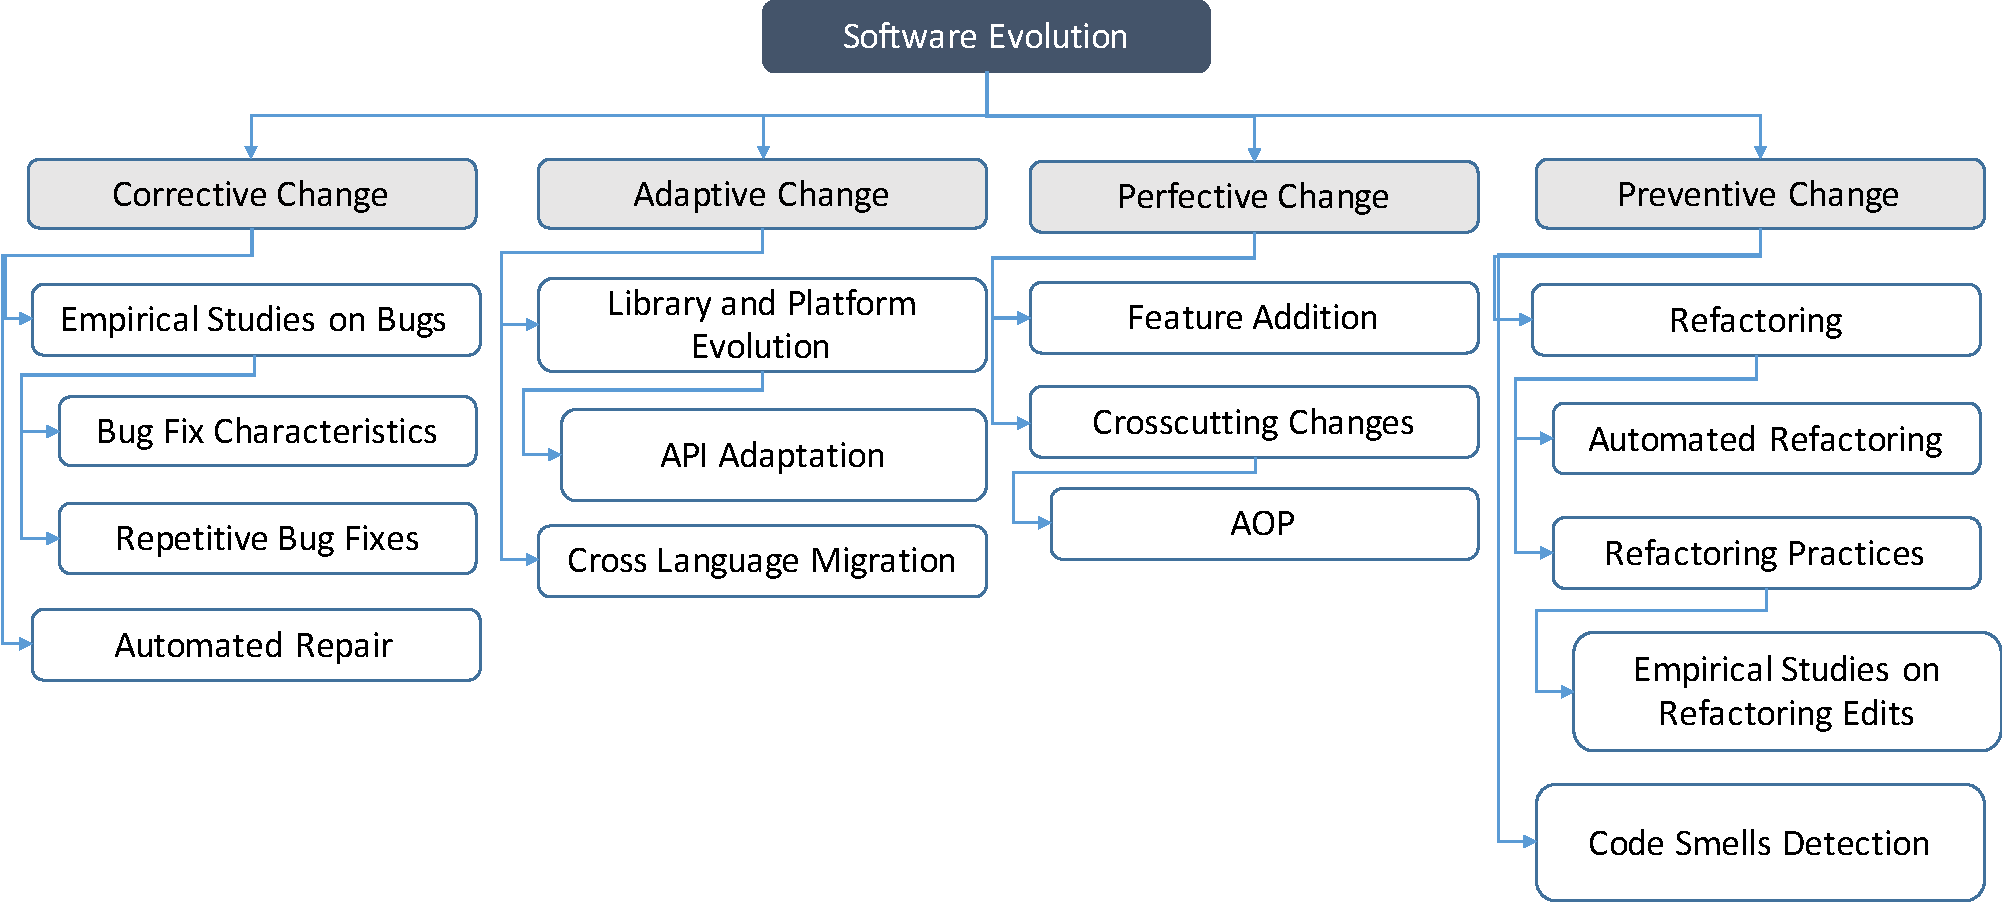
\includegraphics[width=0.95\textwidth]{images/ChangeTypesTopics.pdf}
 \caption{Change Types and Related Research Topics} 
 \label{fig:changetypetopic}
\end{figure}


\subsection{Classifying Software Changes}
\label{sec:classification} 
Swanson initially identified three categories of software changes: corrective, adaptive, and perfective~\cite{Swanson1976:Dimension}. These categories were updated later and ISO/IEC 14764 instead presents four types of changes: corrective, adaptive, perfective, and preventive~\cite{iso}.

\subsubsection{Corrective Change} 
Corrective change refers software modifications initiated by software defects. A defect can result from design errors, logic errors, and coding errors~\cite{Longstreet1990:smc}.

\begin{itemize}
\item Design errors: software design does not fully align with the requirement specification. The faulty design leads to a software system that either incompletely or incorrectly implements the requested computational functionality. 
\item Logic errors: a program behaves abnormally by terminating unexpectedly or producing wrong outputs. The abnormal behaviors are mainly due to flaws in software functionality implementations.
\item Coding errors: although a program can function well, it takes excessively high runtime or memory overhead before responding to user requests. Such failures may be caused by loose coding, or the absence of {\em reasonableness checks} on computations performed.
\end{itemize}

\subsubsection{Adaptive Change}

Adaptive change is a change introduced to accommodate any modifications in the environment of a software product. The term \textbf{environment} here refers to the totality of all conditions that influence the software product, including business rules, government policies, and software and hardware operating systems. For example, when porting a mobile application from Android to iOS, mobile developers need to apply adaptive changes to translate the code from Java to Swift, so that the software is still compilable and executable on the new platform. Programs may be also changed as a result of a new compiler, which performs additional optimizations to generate smaller and faster code. 

%when maintaining a legacy system that was written in Fortran decades ago, programmers may migrate the system to a mainstream general purpose language, such as Java, to facilitate the maintenance of existing codebase and to extend the system by leveraging new features of the popular language. When building phone apps, Mobile developers may port a mobile application from one platform (e.g., Android) to another (e.g. iOS) by translating code from Java to Swift. 
\subsubsection{Perfective Change}

Perfective change is the change undertaken to expand the existing requirements of a system~\cite{Seaman2008:SMC}. When a software product becomes useful, users always expect to use it in new scenarios beyond the scope for which it was initially developed. Such requirement expansion causes changes to either enhance existing system functionality or to add new features. For instance, an image processing system is originally developed to process JPEG files, and later goes through a series of perfective changes to handle other formats of images, such as PNG and SVG.

\subsubsection{Preventive Change}

Preventive change is the change applied to prevent malfunctions or to improve maintainability of software. 
According to Lehman's laws of software evolution~\cite{Lehman1984:ULE}, the long-term effect of corrective, adaptive, and perfective changes is deteriorating the software structure, while increasing entropy. Preventive changes are usually applied to address the problems. For instance, after developers fix some bugs and implement new features in an existing software product, the complexity of source code can increase to an unmanageable level. Through code refactoring---a series of behavior-preserving changes, developers can reduce the code complexity, and increase both readability and reusability of software.
\begin{figure}[!htb]
\centering
\scalebox{0.5}{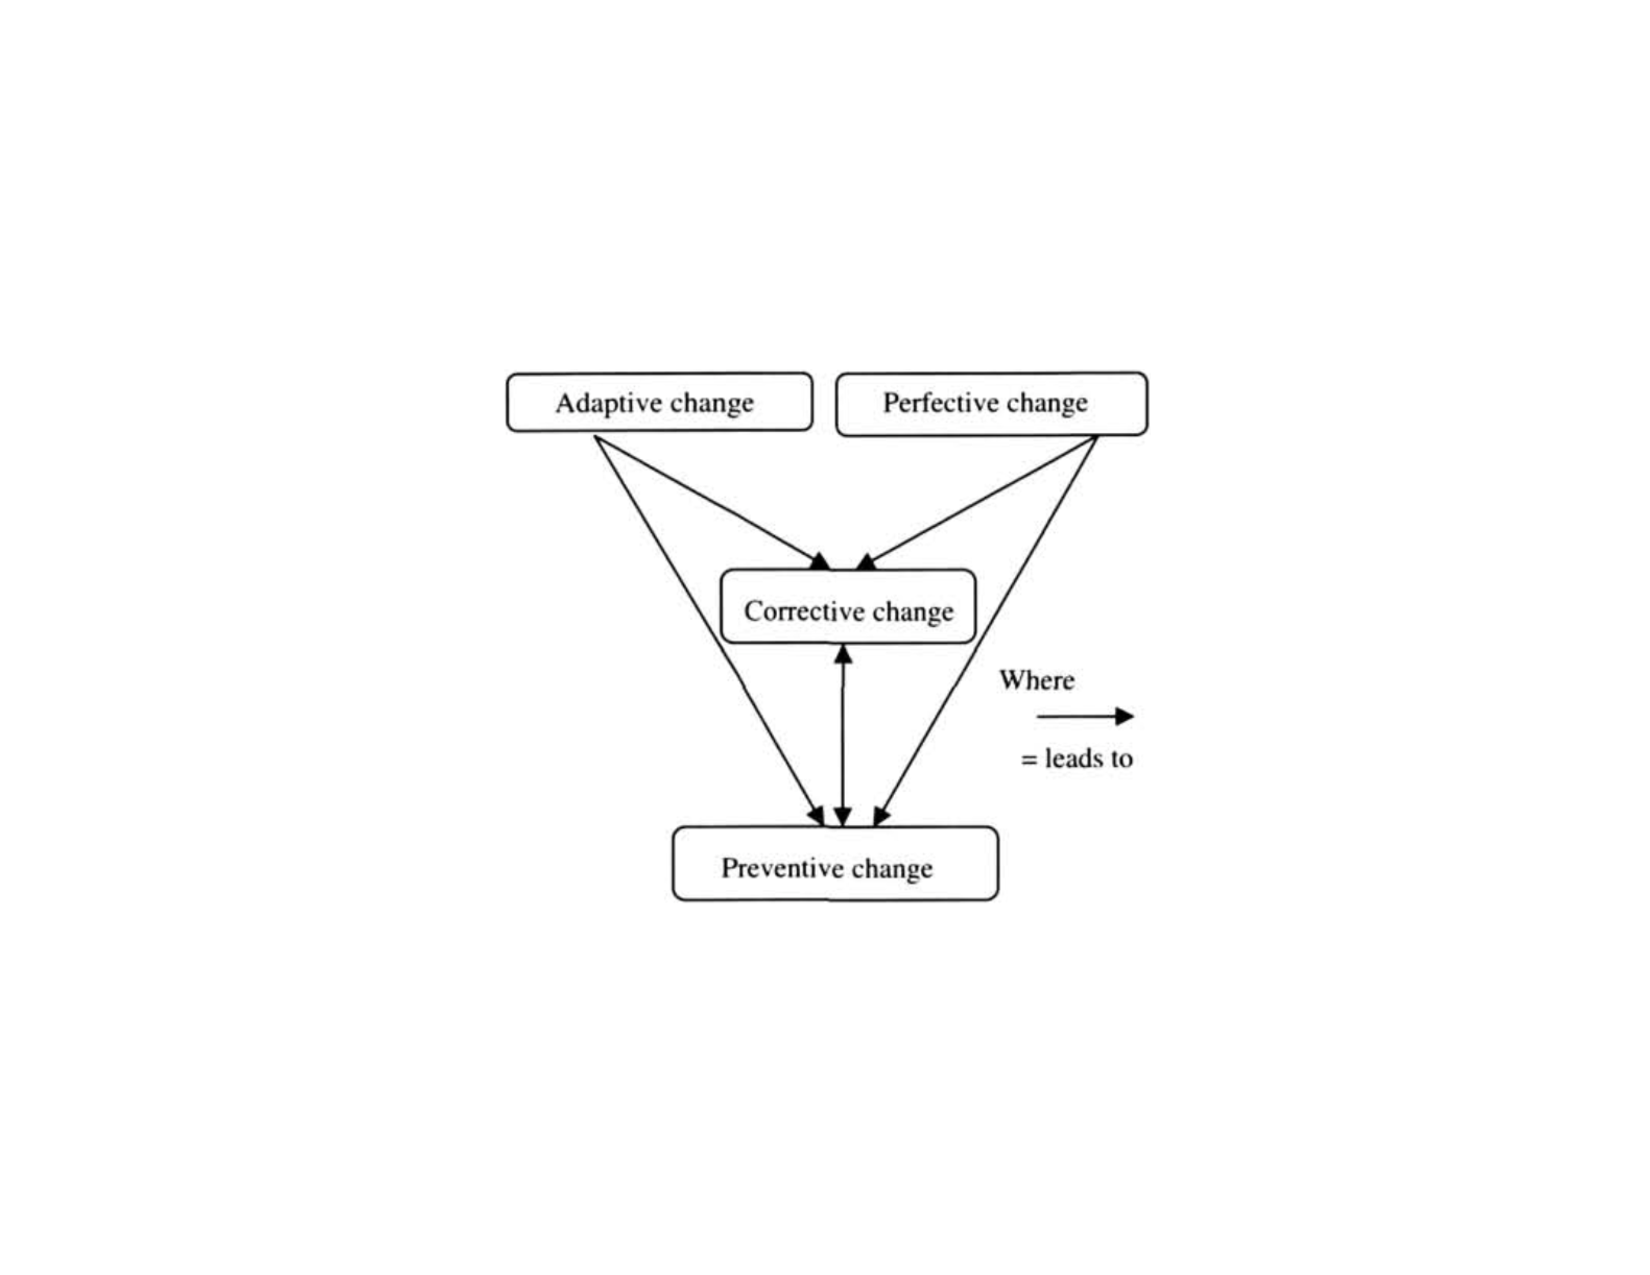
\includegraphics{images/relationship_of_changes.pdf}}
\caption{Potential relation between software changes~\cite{Seaman2008:SMC}}
\label{fig:relation}
\end{figure}

Figure~\ref{fig:relation} presents the potential relationships between different types of changes~\cite{Seaman2008:SMC}. Specifically, both adaptive changes and perfective changes may lead to the other two types of changes, because developers may introduce bugs or worsen code structures when adapting software to new environments or implementing new features.

\subsection{Three Activity Perspectives} 
\label{sec:activity} 
We view the task of evolving software from three activity perspectives: (1) change application, (2) change inspection, and (3) change validation. First, the process of {\em applying} software changes could be further categorized into manual changes vs. automated change application with tool support. In the following three sections, we provide an organized tour of seminal papers focusing on the above-mentioned three kinds of activity perspectives. 

In Section~\ref{sec:apply}, we overview research topics for each of the 4 change types in Section~\ref{sec:classification}. We discuss empirical studies to discuss the characteristics of software changes for each type and overview tool support for applying software changes. For example, for the type of {\em corrective changes}, we present several empirical studies on bug fixes and summarize the characteristics of bug fixes. We then discuss automated techniques for fixing bugs. Similarly, for the type of {\em preventative changes}, we present empirical studies on refactoring practices and refactoring edits and then discuss automated techniques for applying refactorings.  Regardless of change types, various approaches are proposed to reduce the manual effort of updated software through automation. We thus discuss automated change application techniques including source-to-source program transformation, Programming by Demonstration (PbD), simultaneous editing, and systematic editing.

In Section~\ref{sec:inspect}, we overview research topics for inspecting software changes after the corresponding program modifications are made. Software engineers other than the change author perform peer reviews based on their understanding of program changes, and provide feedback if they discover any suspicious software modifications. Therefore, we summarize modern code review processes and discuss techniques for analyzing and understanding code changes. This section overviews a variety of program differencing techniques that developers can use to comprehend code changes and also other types of techniques that raise the abstraction level of program modifications in order to better support the change comprehension and inspection process. 

In Section~\ref{sec:debugtest}, we overview research techniques for validating software changes using debugging, testing, and impact analysis techniques. After software modification is made, developers and testers may create new tests or reuse existing tests based on the requirements specification, run the modified software against the tests, and check whether the software executes as expected. Therefore, the activity of checking correctness about software changes could involve failure-inducing change isolation, regression test selection, and change impact analysis. 


\section{An Organized Tour of Seminal Papers: I. Applying Changes}
\label{sec:apply}

For each of the four types of software changes mentioned in Section~\ref{sec:concepts}, we discuss the characteristics of changes using empirical studies and the process and techniques for applying software changes in Sections~\ref{sec:corrective}-\ref{sec:preventive}. Next, regardless of change types, automated change application could reduce the manual effort of applying software changes. Therefore, we discuss the topic of automated program transformation and editing techniques for reducing repetitive edits in Section~\ref{sec:automatic}.

\subsection{Corrective Change}
\label{sec:corrective}
Corrective changes such as bug fixes are frequently applied by developers to eliminate defects in software. There are mainly two lines of research conducted: empirical studies to characterize bugs or corresponding fixes~\cite{Fenton2000:QAF,Li2006:TCE,Kim2006:MBF,Lu2008:LMC,Nguyen2010:RBF,Yin2011:FBB,Park2012:supplementary,Zhong2015:ESR}, and automatic approaches to help developers detect and fix bugs~\cite{Engler2000:CSR,Bush2000:SAF,Hangal2002:TDS,Hovemeyer2004:FBE,Naik2006:ESR,Weimer2009:AFP}. There is no clear boundary between the two lines of research, because some prior work~\cite{Li2006:CPMiner,Pham2010:DRS,Jin2012:UDR,Kim2013:PAR} did leverage the characteristics observed in empirical studies to automatically detect and fix bugs.

\subsubsection{Empirical Studies of Bug Fixes}
To analyze bug characteristics, Li et al.~conducted an empirical study on bugs from two popular open source projects: Mozilla and Apache HTTP Server~\cite{Li2006:TCE}. By manually examining 264 bug reports from the Mozilla Bugzilla database~\cite{mozilla}, and 209 bug reports from the Apache Bugzilla database~\cite{asf}, they investigated the root cause, impact, and software components of each software error that exhibited abnormal runtime behaviors. They observed three major root causes: memory, concurrency, and semantics. The memory bugs account for 16.3\% in Mozilla and 12.2\% in Apache. Among memory bugs, NULL pointer dereference was observed as a major cause, accounting for 37.2 to 41.7\%. More importantly, semantic bugs are observed to be dominant, accounting for 81.1\% in Mozilla and 86.7\% in Apache. One possible reason is that most semantic bugs are specific to applications. A developer can easily introduce semantic bugs while coding, due to a lack of thorough understanding of the software. It is challenging to automatically detect or fix such bugs, because diagnosing and resolving them may require a lot of domain-specific knowledge.

To characterize bug fixes, Kim et al.~conduct an empirical study on bug fixing data from the change history of five open source projects: ArgoUML, Columba, Eclipse, jEdit, and Scarab~\cite{Kim2006:MBF}. With keywords like ``Fixed'' or ``Bugs'', they retrieved code commits in software version history that are relevant to bug fixes, chopped each commit into contiguous code change blocks (i.e., hunks), and then clustered similar code changes. They observed that 19.3 to 40.3\% bugs appeared repeatedly in version history, while 7.9 to 15.5\% of bug-and-fix pairs appeared more than once. The results demonstrate that project-specific bug fix patterns occur frequently enough to be useful as a bug detection technique. Furthermore, for the bug-and-fix pairs, it is possible to both detect the bug and provide a strong suggestion for the fix. 

\begin{table}[]
\centering
\caption{Sample system rule templates and examples from~\cite{Engler2000:CSR}}
\label{tab:rule}
\begin{tabular}{l|l}
\toprule
Rule template                  & Example                                                 \\ \hline
``Never/always do X''          & ``Do not use floating point in the kernel''             \\\hline
``Do X rather than Y''         & ``Use memory mapped I/O rather than copying''           \\ \hline
``Always do X before/after Y'' & ``Check user pointers before using them in the kernel''\\
\bottomrule
\end{tabular}
\end{table} 

\subsubsection{Automatic Bug Detection and Fixing Approaches}
Engler et al.~defined a meta-language for users to easily specify temporal system rules such as ``release locks after acquiring them''~\cite{Engler2000:CSR}. They also extended a compiler to interpret the rules and dynamically generate additional checks in the compiler. If any code snippet violates the specified rule(s), the approach reports the snippet as a software bug. Table~\ref{tab:rule} presents some exemplar system rule templates and instances. 
With this approach, developers can flexibly define their own rules to avoid some project-specific bugs, without worrying how to implement checkers to enforce the rules.

Li et al. developed CP-Miner, an automatic approach to find copy-paste related bugs in large-scale software~\cite{Li2006:CPMiner}. CP-Miner was created based on a prior empirical study~\cite{Chou2001:ESO}, which revealed that under the Linux {\sf drivers/i2o} directory, 34 out of 35 errors were caused by copy-paste or duplicated code. 
One of the major reasons why copy-paste introduces bugs is that when developers copy code from one location and paste it to another location, they forget to consistently rename identifiers of variables, functions, and types. CP-Miner first identifies copy-paste code in a scalable way, and then detects bugs associated with copy-paste by checking the renamed identifiers. If an identifier is inconsistently renamed, with some of its occurrences replaced and some not replaced, CP-Miner reports it as a copy-paste bug. Many previously unknown bugs in popular operating systems were detected in this way, 49 in Linux and 31 in FreeBSD, meaning that CP-Miner can effectively capture copy-paste related bugs. 


\subsubsection{Automated Repair.} 

Automatic program repair generates candidate patches and checks correctness using compilation and testing~\cite{Weimer2009:repair}.  For example, Weimer et al.~generate candidate patches by replicating, mutating, or deleting code \emph{randomly} from the existing program. They do not infer edits from multiple edit examples, nor do they systematically apply an edit to multiple places. Specification-based program repair such as AutoFix-E~\cite{Wei:2010:AutoFix-E} generates simple bug fixes from manually prescribed contracts. FixMeUp inserts missing security checks interprocedurally using a specification, but these additions are very specific and stylized~\cite{SMS:13}.  
Kim et al.'s PAR~\cite{Kim2013:PAR} use ten common bug fix patterns inferred from Eclipse JDT's version history to improve the patch suggestions of Weimer et al.~\cite{Weimer2009:repair}. However, the patterns are created manually. Since systematic editing techniques such as LASE automate bug fix pattern inference and when used together with PAR, it could reduce manual effort of similar bug fixes significantly. Given concurrency error reports, Jin et al. select from and test a handful of synchronization patterns to fix them~\cite{JZDLL:12}. They insert appropriate synchronization into a compiler intermediate representation, whereas LASE~\cite{Meng2013:lase} directly modifies the program. Although LASE does not coordinate cross method or interprocedural changes, it handles a much larger class of edits than all these tools. 

One class of strategies in automatic software repair relies on specifications or contracts to guide sound patch generation~\cite{gopinath2011, liblit2011, liu2012, semfix13, zeller2010}. This provides confidence that the output is correct.  Genetic programming has also been used to co-evolve defect repairs and unit test cases~\cite{Arcuri11,wilkerson2012}; these techniques tend to rely at least in part on formal specifications to define correctness~\cite{arcuriy08,wilkerson11}.  Such techniques struggle to scale, and are usually limited to manually specified code, which is rare in practice.

Another set of techniques uses search-based software engineering~\cite{harman07} or predefined repair templates to generate many candidate repairs for a bug, and then validates them using indicative workloads or test suites~\cite{Kim2013:PAR, genprog-icse2012, Perkins09:clearview}.  Many of these approaches can scale to repair defects in large systems with human-competitive costs.  However, they tend to find the smallest possible fix for a given failure, and current evidence suggests that humans may find the resulting patches unacceptable in many cases~\cite{genprog-maintainability,Kim2013:PAR}. 

\subsection{Adaptive Change}
\label{sec:adaptive}

Adaptive changes are applied to a software product, when its environment changes. In this section, we focus on two scenarios when adaptive changes are applied: software library upgrade and cross-language software migration.
\todo{Na, don't we need to describe changes coming from environment changes more broadly? I think it would make sense to include a category of feature addition. It seems to be the two categories of library update and cross-language transformation seem too narrow in its focus and not comprehensive enough to describe various kinds of software changes. Could we add a new category of platform update, changes to improve performance, etc?} 


\subsubsection{Library and Platform Evolution} 
When building new software (e.g., a search engine), instead of coding everything from scratch, developers always extend existing frameworks or third-party libraries (e.g., Lucene~\cite{lucene}) by invoking the Application Programming Interfaces (APIs), to reuse the well implemented and fully tested functionality. However, as library developers release new versions of their software to fix existing bugs and include new features, client developers should also upgrade the libraries used in their projects to benefit from the newer versions. Ideally, the library APIs should be stable so that such software upgrades do not incur any program change in client applications. In reality, nevertheless, these APIs are susceptible to changes, requiring client developers to apply adaptive changes for the usage of new library versions. 

\begin{figure}
\centering
\scalebox{0.4}{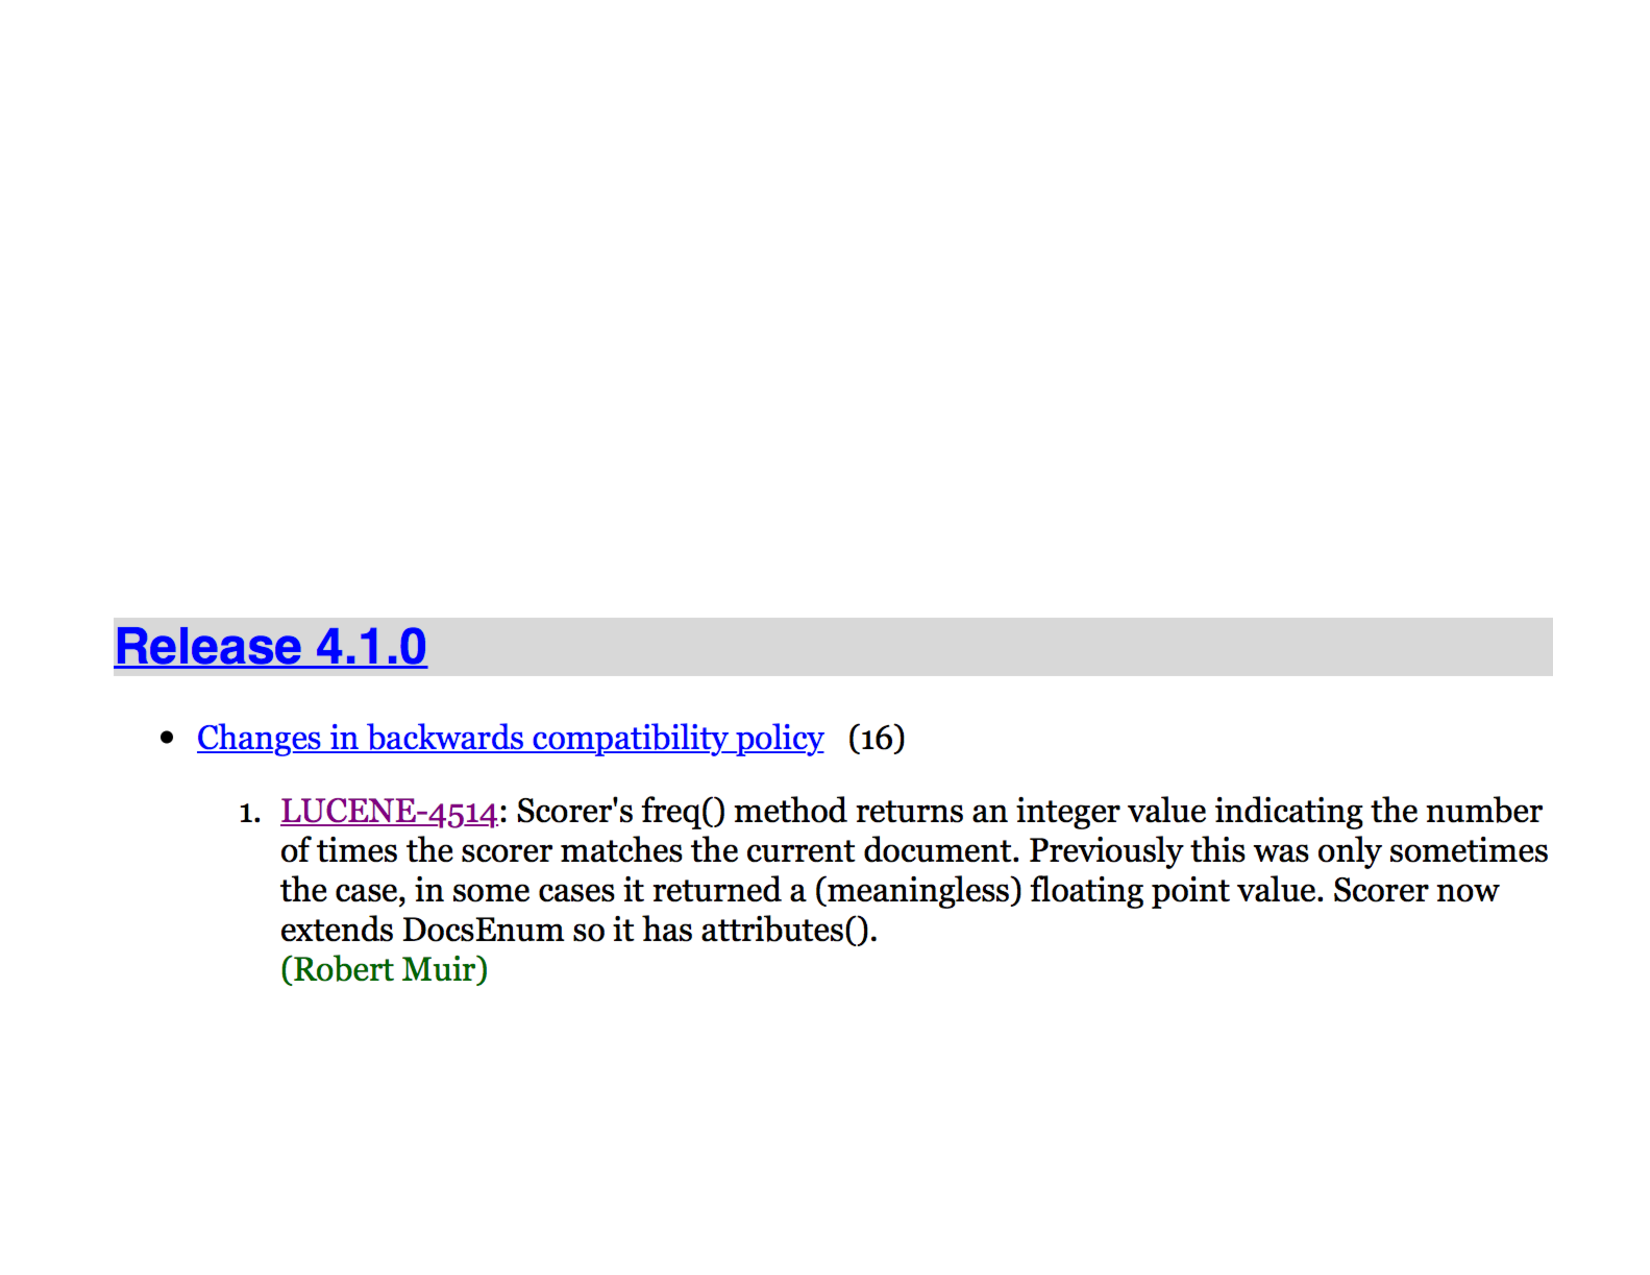
\includegraphics{images/releasenote.pdf}}
\caption{An excerpt of the Lucene change log for Release 4.1.0~\cite{releasenote}}
\label{fig:releasenote}
\end{figure}

\paragraph{Empirical Studides of API Evolution} 
Dig and Johnson \cite{Dig2005} manually investigated API changes using the change logs and release notes to study the types of library-side updates that break compatibility with existing client code, and discovered that 80\% of such changes are refactorings. Xing and Stroulia~\cite{Xing2006:apievol} used UMLDiff to study API evolution in several systems, and found that about 70\% of structural changes are refactorings. Kim et al.'s signature change pattern analysis \cite{Kim2006:apievol} categorizes API signature changes in terms of data-flow invariant. Yokomori et al.~\cite{Yokomori2009:apiimpact} investigated the impact of library evolution on client code applications using component ranking measurements. Padioleau et al.~\cite{Padioleau2006} found that API changes in the Linux kernel lead to subsequent changes on dependent drivers, and such collateral evolution could introduce bugs into previously mature code. These studies motivate the need for supporting complex client adaptations beyond replaying library-side refactorings in client code.  

\paragraph{API Stability} 
\todo{ICSM 2013: android study}

\paragraph{Tool Support for API Evolution and Client Adaptation} 
There are several existing approaches to support client adaptations to cope with evolving libraries.  Chow and Notkin~\cite{Chow1996} proposed a method for changing client applications in response to library changes\textemdash a library maintainer annotates changed functions with rules that are used to generate tools that will update client applications. Henkel and Diwan's CatchUp~\cite{Henkel2005} records and stores refactorings in an XML file that can be replayed to update client code. However, its update support is limited to three refactorings: renaming operations (e.g.  types, methods, fields), moving operations (e.g. classes to different packages, static members), or change operations (e.g. types, signatures). The key idea of CatchUp, {\em record-and-replay}, assumes that the adaptation changes in client code are exact or similar to the changes in the library side. Thus, it works well for replaying rename or move refactorings or supporting API usage adaptations via inheritance. However, CatchUp cannot suggest programmers how to manipulate the context of API usages in client code such as the surrounding control structure or the ordering between method-calls such as the example shown in Section~\ref{sec:empirical}. Furthermore, CatchUp requires that library and client application developers use the same development environment to record API-level refactorings, limiting its adoption in practice.

SemDiff~\cite{Dagenais2008} mines API usage changes from other client code or the evolution of library itself, similar to our work.  The key difference of {LibSync} from SemDiff is that with our work uses a graph-based representation to capture the context of an API usage, including the dependencies among method calls and with a surrounding control logic. In our work, an adaptation pattern is captured in term of a frequent set of graph editing operations that are common to multiple API usage skeletons before and after library migration. On the other hand, SemDiff defines an adaptation pattern as a frequent {\em replacement} of a method invocation. That is, if a method call to $A.m$ is changed to $B.n$ in several adaptations, $B.n$ is likely to be a correct replacement for the calls to $A.m$. As SemDiff models API usages in terms of method calls, it cannot support complex adaptations that involve multiple objects and method calls and that require the knowledge of the surrounding context of those calls. {LibSync}'s key departure point is that when a library's API declarations are modified, such evolution often involves coordinating uses of multiple objects and multiple method calls under certain contexts.

Xing and Stroulia's Diff-CatchUp~\cite{Xing2007:diffcatchup} automatically recognizes API changes of the reused framework and suggests plausible replacements to the obsolete APIs based on working examples of the framework codebase.  Dig et al.'s MolhadoRef~\cite{Dig2007} uses recorded API-level refactorings to resolve merge conflicts that stem from refactorings; this technique can be used for adapting client applications in case of simple rename and move refactorings occurred in a library.  

Tansey and Tilevich's approach~\cite{Tansey2008:annotation} infers generalized transformation rules from given examples so that application developers use the inferred rules to refactor legacy applciations. However, this approach focuses on annotation refactorings that replace the type and naming requirements to the annotation requirements of a target framework. Furthermore, this approach does not focus on updating client applications to cope with evolving libraries. 

Andersen and Lawall~\cite{Andersen2008:patch} proposed {\em spdiff} that identifies common changes made in a set of files.  API developers could use {\em spdiff} to extract a generic patch and apply it to other clients. Their approach models the changes at the level of {\em text-line} changes. On the other hand, {LibSync} uses a graph-based representation to capture more thorough syntactic and semantic information for adapting API usages.  SmPL~\cite{Padioleau2007,Lawall2009:apienforce} is a domain-specific source transformation language that captures textual patches with a more semantic description of program changes. However, it does not explicitly distinguish API changes from their usage changes. 

\paragraph{API Usage Specification Extraction} 
There exist several approaches for extracting API usage specifications. The forms of recovered API usage specifications and patterns include finite state automaton~\cite{zeller07,haozhong09}, pairs of method calls~\cite{dynamine05,williams-tse05}, partial orders of calls~\cite{mapo-fse07,taoxie-ase09}, Computation Tree Logic formulas~\cite{zeller-ase09}. The API usage representations in those static approaches are still limited, for example, the patterns are without control structures and involve only individual objects belonging to one class. Our graph-based API usage representation captures multi-object API usage patterns with control structures. In contrast to those static approaches, dynamic approaches recover the specifications by investigating the execution traces of programs~\cite{javert08,yang-icse06,shoham-issta07,ramanathan-isce07,mike-ase09}.  These dynamic approaches require a huge amount of execution traces.  Our graph-based representation, iGROUM, captures API usage patterns with control and data dependencies among method calls, and surrounding control logic such as \codefont{while} loop and \codefont{if} statement. 
The API usage representations in this paper extend our prior work on GRouMiner~\cite{fse09} to tailor the original multi-object usage representation in order to capture the relevant context surrounding the use of external APIs. In particular, iGROUM explicitly captures API types and methods that appear in action and data nodes, so that program slicing can isolate only a sub-graph that is relevant to the use of a particular library. We also created a new model called xGROUM to represent overriding and inheritance relationships between client methods and API methods. 


\subsubsection{Cross-language Migration} 
When maintaining a legacy system that was written in an old programming language (e.g., Fortran) decades ago, programmers may migrate the system to a mainstream general-purpose language, such as Java, to facilitate the maintenance of existing codebase and to extend the system by leveraging new features of the popular language. Different from the API adaptive changes mentioned above, such software translation requires of a significant amount of coding effort to rewrite the same application in a new programming language.

TXL is a source transformation language designed to translate or manipulate programming languages~\cite{Cordy2006}. As shown in Figure~\ref{fig:txl}, a typical TXL file consists of two parts. The first part defines a context-free grammar to describe program syntax, while the second part describes a set of transformation rules to manipulate the syntax. For our illustrative example, the grammar defines a simple language that only allows numbers, addition and subtraction numerical expressions. The rule \codefont{resolveAddition} describes the resolution of an addition expression by replacing the expression with a number value \codefont{N1 [ + N2 ]}. Given such a file, the TXL program transformation engine automatically transforms programs of the syntactic structure by applying the rules. 

\begin{figure}
\centering
\scalebox{0.5}{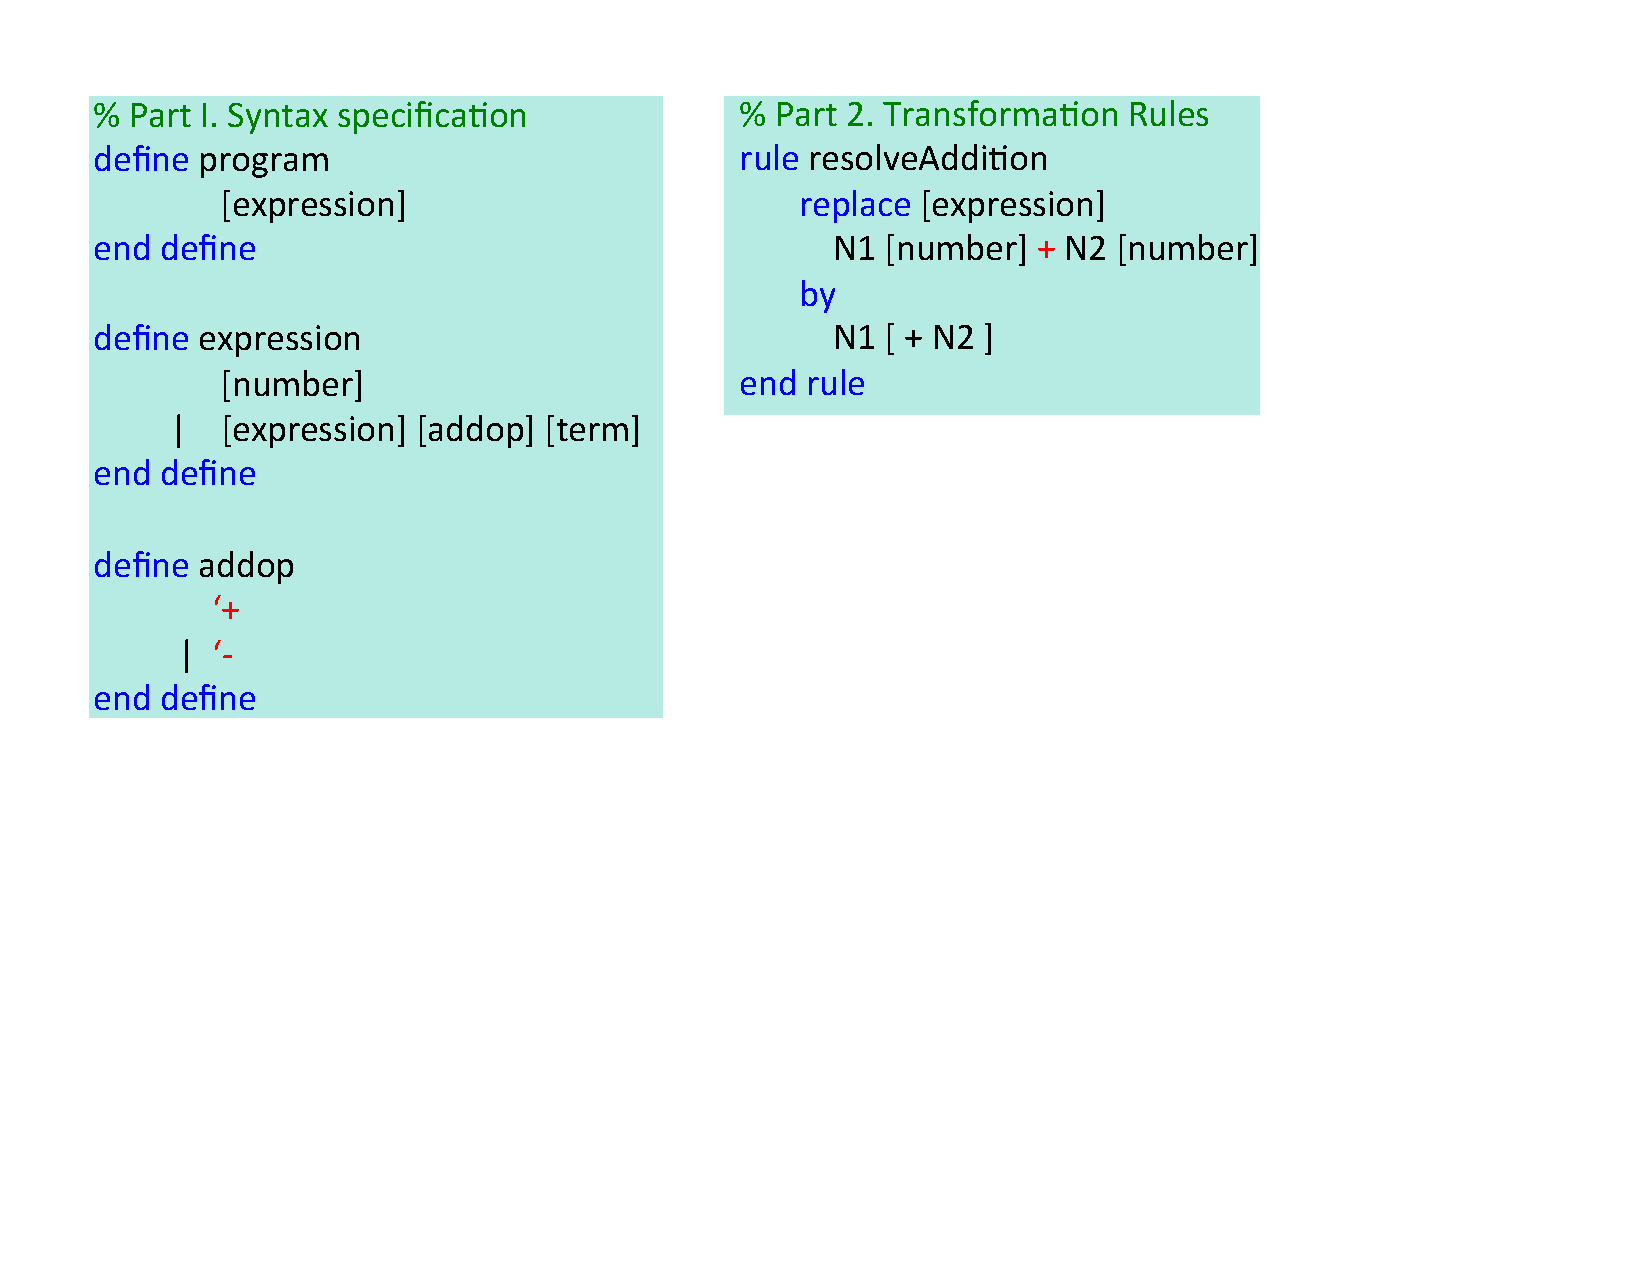
\includegraphics{images/txl.pdf}}
\caption{A simple exemplar TXL file based on~\cite{txltour}}
\label{fig:txl}
\end{figure}
With TXL, developers to not need to build programming language translators by coding every line of implementation. Instead, the transformation engine can automatically translate code once developers specify all needed grammars and rules. Researchers built tools using TXL to automate various code translation tasks, like ASP-to-NSP and Java-to-C\#~\cite{Chu:08,Hassan:2005,El-Ramly:2006,Tonella:04}.

\subsubsection{Cross-System Porting} 
\todo{FSE 2012} 



\subsection{Perfective Change}
\label{sec:perfective}

\subsubsection{Crosscutting Changes} 

As programs evolve over time, they may suffer from the {\it the tyranny of dominant decomposition} \cite{Tarr1999}. They can be modularized in only one way at a time. Concerns that are added later may end up being scattered across many modules and tangled with one another.  Logging, performance, error handling, and synchronization are canonical examples of such secondary design decisions.  These can be seen as another kind of systematic change that involves inserting similar code throughout a program.  Aspect-oriented programming languages provide language constructs to allow concerns to be updated in a modular fashion \cite{Kiczales2001}. A number of other approaches instead leave the crosscutting concerns in a program while providing mechanisms to manage related but dispersed code fragments.  Griswold's information transparency technique uses naming conventions, formatting styles, and ordering of code in a file to provide indications about code that should change together \cite{Griswold2001}. 

There are several tools that allow programmers to automatically or semi-automatically locate crosscutting concerns. Robillard et al. \cite{Robillard2003} allow programmers to manually document crosscutting concerns using structural dependencies in code. Similarly, the Concern Manipulation Environment \cite{Harrison2005} allows programmers to locate and document different types of concerns. 
Van Engelen et al. \cite{VanEngelen2005} use clone detectors to locate crosscutting concerns. Shepherd et al. \cite{Shepherd2007} locate concerns using natural language program analysis.  Breu et al. \cite{Breu2006} mine aspects from version history by grouping method-calls that are added together. Dagenais et al. \cite{Dagenais2007} automatically infer and represent structural patterns among the participants of the same concern as rules in order to trace the concerns over program versions. In general, our change-rule inference techniques differ from these tools by inferring general kinds of systematic changes, which may or may not be crosscutting concerns, and by detecting anomalies from systematic changes. 

Developers apply perfective changes when enhancing or adding software features by implementing new code. There is not much research done in this area to facilitate feature enhancement or addition. One possible reason is that the implementation logic is always project-specific and spontaneous. It is challenging for any automatic tool to predict what new code to add, and to suggest what rules to apply when integrating new code with existing codebases. In this section, we mainly focus on two most closely relevant research topics: Aspect Oriented Programming (AOP) and Feature Oriented Programming (FOP).

\paragraph{AOP} is a programming paradigm that aims to increase modularity by allowing the separation of cross-cutting concerns~\cite{Kiczales1997}. Suppose developers want to add a new feature---logging---to log all executed functions. 
The logging logic is straightforward: printing the function's name at each function's entry. However, manually inserting the same implementation to each function body is tedious and error-prone. With AOP, developers only need to first define the logging logic as \textbf{an advice}, and then specify the place where to insert the advice (i.e., \textbf{pointcut}), such as the entry point of each function. An aspect weaver will read the aspect-oriented code, and generate appropriate object-oriented code with the aspects integrated. In this way, AOP facilitate developers to efficiently introduce new program behaviors without cluttering the core implementation in the existing codebase. Many Java bytecode manipulation frameworks implement the AOP paradigm, like ASM~\cite{asm}, Javassist~\cite{javassist}, and AspectJ~\cite{aspectj}, so that developers can easily modify program runtime behaviors without touching the source code. 


\paragraph{FOP} is a paradigm for program generation in software product lines and for incremental development of programs~\cite{Batory1992:DIH}. 
FOP is closely related to AOP. Both deal with modules that encapsulate crosscuts of classes, and both express program extensions.
In FOP, every software is considered as a composition of multiple features or layers. Each feature implements a certain program functionality, while features may interact with each other to collaboratively provides a larger functionality or get adapted to each other.
A software product line (SPL) is a family of programs where each program is defined by a unique composition of features. Formally, FOP considers programs as \emph{values} and program extensions as \emph{functions}~\cite{Lammel2013:fop}. Suppose there are two programs: 

$f \text{	// program with feature }f$, and

$g\text{	// program with feature }g$.

\noindent
A program extension is a function that takes a program as input and produces a feature-augmented program output. Suppose there are two program extensions:

$i \bullet x$ // adds feature i to program x, and 

$j \bullet y$ // adds feature j to program y.

By applying the functions to the values, we can compose more than one multi-featured application as below:

$app1 = i \bullet f$ // app1 has features i and f,

$app2 = j \bullet g$ // app2 has features j and g, and
 
$app3 = i \bullet j \bullet f$ // app3 has features i, j, f.

 
 

\subsection{Preventive Change}
\label{sec:preventive}

As a software system is enhanced, modified, and adapted to new requirements, the code becomes more complex and drifts away from its original design, thereby lowering the quality of the software. {\bf Refactoring (Restructuring)} \cite{Fowler2000, Griswold1991, Opdyke1992, Mens2004} copes with increasing software complexity by transforming a program from one representation to another while preserving the program's external behavior (functionality and semantics).% {\it Refactoring} is another name for restructuring, usually in the context of object-oriented programming languages \cite{Opdyke1992}. 

Griswold's dissertation \cite{Griswold1991} discusses one of the first refactoring tools that automate repetitive, error-prone, non-local transformations. Griswold's tool supports a number of restructuring operations: replacing an expression with a variable that has its value, swapping the formal parameters in a procedure's interface and the respective arguments in its calls, etc. It is important to note that many of these restructurings are systematic in the sense that they involve repetitive non-local transformations. 

Opdyke's dissertation \cite{Opdyke1992} distinguishes the notion of low-level refactorings from high-level refactorings. High-level refactorings (i.e., composite refactorings) reflect more complex behavior-preserving transformations while low-level refactorings are primitive operations such as creating, deleting, or changing a program entity or moving a member variable. Opdyke describes three kinds of complex refactorings in detail: (1) creating an abstract superclass, (2) subclassing and simplifying conditionals, and (3) capturing aggregations and components. All three refactorings are systematic in the sense that they contain {\bf \em multiple} similar transformations at a code level. For example, {creating an abstract superclass} involves moving {\bf \em multiple} variables and functions common to {\bf \em more than one} sibling classes to their common superclass.  {Subclassing and simplifying conditionals} consists of creating {\bf \em several} classes, each of which is in charge of evaluating a different conditional.  {Capturing aggregations and components} usually involves moving {\bf \em multiple} members from a component to an aggregate object. 

While refactoring is defined as behavior-preserving code transformations in the academic literature~\cite{Mens2004}, the de-facto definition of refactoring in practice seems to be very different from such rigorous definition. Fowler catalogs 72 types of structural changes in object oriented programs but these transformations do not necessarily guarantee behavior preservation~\cite{Fowler2000}. In fact, Fowler recommends developers to write test code first before, since these refactorings may change a program's behavior. Murphy-Hill et al.~analyzed refactoring logs and found that developers often interleave refactorings with other behavior-modifying transformations~\cite{Murphy-Hill2009:refactor}, indicating that pure refactoring revisions are rare. Johnson's refactoring definition is aligned with these findings\textemdash{\it refactoring improves behavior in some aspects but does not necessarily preserve behavior in all aspects}~\cite{Johnson2011}. A field study of refactoring in industry~\cite{Kim2014:microsoft,Kim2012:fieldrefactoring} finds that refactoring is not confined to low-level, semantics-preserving transformations from developers' perspectives.    




Typically, a refactoring process consists of the following activities~\cite{Mens2004:SSR}:
\begin{enumerate}
\item Identifying where to apply what refactoring(s).
\item Checking that the refactoring to apply preserves program behaviors.
\item Refactoring the code.
\item Assessing the effect of applied refactoring on software quality (e.g., complexity and readability). 
\item Maintaining the consistency between refactored code and other related software artifacts, like documentation, tests, and issue tracking records.  
\end{enumerate}

Researchers have proposed different approaches, techniques, or formalisms to support each of above activities.
%Researchers proposed various approaches to automate refactoring or to complete the refactoring tasks initiated by developers~\cite{Griswold:1992,Balazinska1999,Dig:2009,Ge:2012,Chen:2013,Lee:2013,Tsantalis2013:icsm,Meng:2015,Kim:2016}. Eclipse IDE also provides tool support to automate some of the refactorings mentioned in Fowler's catalog, such as \emph{Extract Method}, \emph{Pull up Method}, and \emph{Move Field}. 

\subsubsection{Automated Refactoring} 

The Eclipse IDE provides automatic support for a variety of refactorings, including \emph{rename}, \emph{move}, and \emph{extractMethod}. With such support, developers do not need to worry about how to check for preconditions or postconditions before manually applying a certain refactoring. Instead, they can simply select the refactoring command from a menu (e.g., \emph{extractMethod}), and provide necessary information to accomplish the refactoring (e.g., method name). The Eclipse refactoring engine takes care of the precondition check, program transformation, and postcondition check. Additionally, 
researchers conducted empirical studies to characterize the refactorings applied by developers~\cite{Kim2012:FSR,Murphy-Hill2012:refactor,Vailian2012:misuse,Silva2016:WWR}, and proposed various approaches to automate refactoring or to complete the refactoring tasks initiated by developers~\cite{Griswold:1992,Balazinska1999,Dig:2009,Ge:2012,Chen:2013,Lee:2013,Tsantalis2013:icsm,Meng:2015,Kim:2016}. For instance, Silva et al.~observed that refactoring activity is mainly driven by changes in the requirements and much less by code smells~\cite{Silva2016:WWR}. Kim et al.~developed R3, an alternative refactoring engine that works 10 times faster than Eclipse Refactoring~\cite{Kim:2016}. 

\todo{Example of Clone Removal Refactoring. RASE ICSE 2015} 

\subsubsection{Empirical Studies of Refactoring} 

Xing and Stroulia found that 70\% of structural changes in Eclipse's evolution history are due to refactorings and existing IDEs lack support for complex refactorings~\cite{Xing2005}. Dig et al.~studied the role of refactorings in API evolution, and found that 80\% of the changes that break client applications are API-level refactorings~\cite{Dig2005}. 

Hindle et al. found that large commits are more perfective (refactorings) while small commits are more corrective (bug fixes)~\cite{Hindle2008}. Purushothaman and Perry found that nearly 10\% of changes involved only a single line of code, which has less than a 4\% chance to result in error, while a change of 500 lines or more has nearly a 50\% chance of causing at least one defect. Though the focus of these studies is different from our study, the results are somewhat aligned with ours: large commits, which tend to include refactorings, have a higher chance of inducing bugs. 

Wei{\ss}gerber and Diehl found that refactorings often occur together with other types of changes and that refactorings are followed by an increasing number of bugs~\cite{Weissgerber2006:refactor}. Carriere et al.'s case study found that the productivity measure manifested by the average time taken to resolve tickets decreases after re-architecting the system~\cite{Carriere2010:architecture}. 
Ratzinger et al. developed defect prediction models based on software evolution attributes and found that refactoring related features and defects have an inverse correlation~\cite{Ratzinger2008:refactor}\textemdash if the number of refactorings increases in the preceding time period, the number of defects decreases.   Our results are aligned with some of these findings, yet improve upon these studies. Our study method not only relates refactorings and bug fixes based on their temporal proximity using a K-revision sliding window but also considers method-level location of refactorings and bug fixes to examine whether bug fixes are related to a preceding refactoring. 

Though the intent of refactoring is to improve software maintainability, refactoring could be potentially error-prone as it often requires coordinated edits across different parts of a system. Several researchers found such evidence from open source project histories\textemdash M. Kim et.al.'s program differencing technique~\cite{Kim2007, Kim2009} identifies exceptions to systematic change patterns, which often arise from the failure to complete coordinated refactorings. G{\"o}rg and Wei{\ss}gerber detect errors caused by incomplete refactorings by relating API-level refactorings to the corresponding class hierarchy~\cite{Weissgerber2006:refactor}. 

\paragraph{Quantitataive Assessment of Refactoring Benefits} 
While several prior research efforts have conceptually advanced our understanding of the benefit of refactoring through metaphors, few empirical studies assess refactoring benefits quantitatively. Sullivan et al.~first linked software modularity with option theories~\cite{Sullivan1998:option}. A module provides an option to substitute it with a better one without symmetric obligations, and investing in refactoring activities can be seen as purchasing \emph{options} for future adaptability, which will produce benefits when changes happen and the module can be replaced easily. Baldwin and Clark~\cite{Baldwin1999:designrule} argued that the modularization of a system can generate tremendous value in an industry, given that this strategy creates valuable options for module improvement. Ward Cunningham drew the comparison between debt and a lack of refactoring: a quick and dirty implementation leaves {\em technical debt} that incur \emph{penalties} in terms of increased maintenance costs~\cite{Cunningham1992:td}. While these projects advanced conceptual understanding of refactoring impact, they do not quantify the benefits of refactoring.  Kim et al.~\cite{Kim2014:microsoft} study on how refactoring impacts inter-module dependencies and defects using the quantitative analysis of Windows 7 version history. Their study finds the top 5\% of preferentially refactored modules experience higher reduction in the number of inter-module dependencies and several complexity measures but increase size more than the bottom 95\%. Based on the hypothesis that measuring the impact of refactoring requires multi-dimensional assessment, they investigate the impact of refactoring on various metrics: churn, complexity, organization and people, cohesiveness of ownership, test coverage and defects.     

MacCormack et al.~\cite{MacCormack2006:study} defined modularity metrics and used these metrics to study evolution of Mozilla and Linux. They found that the redesign of Mozilla resulted in an architecture that was significantly more modular than that of its predecessor. However, unlike our study on Windows, their study merely monitored design structure changes in terms of modularity metrics without identifying the modules where refactoring changes are made. 

Kataoka et al.~\cite{Kataoka2002:metric} proposed a refactoring evaluation method that compares software before and after refactoring in terms of coupling metrics. Kolb et al.~\cite{Kolb2006:refactoring} performed a case study on the design and implementation of existing software and found that refactoring improves software with respect to maintainability and reusability. Moser et al.~\cite{Moser2006:refactoring} conducted a case study in an industrial, agile environment and found that refactoring enhances quality and reusability related metrics. Carriere et al.'s case study found the average time taken to resolve tickets decreases after re-architecting the system~\cite{Carriere2010:architecture}. Ratzinger et al.~developed defect prediction models based on software evolution attributes and found that refactoring related features and defects have an inverse correlation~\cite{Ratzinger2008:refactor}\textemdash if the number of refactoring edits increases in the preceding time period, the number of defects decreases. These studies indicated that refactoring positively affects productivity or quality measurements. Similarly, Tahvildari et al.~suggested using a catalogue of object-oriented metrics to estimate refactoring impact, including complexity metrics, coupling metrics, and cohesion metrics~\cite{Tahvildari2003:MAE}. 

On the other hand, several research efforts found contradicting evidence that refactoring may affect software quality negatively. Wei{\ss}gerber and Diehl found that refactoring edits often occur together with other types of changes and that refactoring edits are followed by an increasing number of bugs~\cite{Weissgerber2006:refactor}.  Kim et al.~found that the number of bug fixes increases after API refactorings~\cite{Kim2011:refactorbug}.  Nagappan and Ball found that code churn\textemdash the number of added, deleted, and modified lines of code\textemdash is correlated with defect density~\cite{Nagappan2005}\textemdash{} since refactoring often introduces a large amount of structural changes to the system, some question the benefit of refactoring. G{\"o}rg and Wei{\ss}gerber detected errors caused by incomplete refactorings by relating API-level refactorings to the corresponding class hierarchy~\cite{Weissgerber2006:refactor}.  

\subsubsection{Empirical Studies of Modern Refactoring Practices} 

{\bf Real-world software enhancements are generally not semantics-preserving and they are beyond the scope and capability of existing refactoring engines.} To investigate the challenges associated with refactorings, we conducted a survey with professional developers at Microsoft~\cite{Kim2012:fieldrefactoring}. We sent a survey invitation to 1290 engineers whose commit messages include a keyword ``refactoring'' in the version histories of five MS products. 328 of them responded to the survey. More than half of the participants said they carry out refactorings in the context of bug fixes or feature additions, and these changes are generally not semantics-preserving. When we asked about their own definition of refactoring, 46\% of participants did not mention preservation of semantics, behavior, or functionality at all. This observation is consistent with Johnson's argument that, while refactoring preserves some behavior, it does not preserve behavior in all aspects~\cite{Johnson2011}. 53\% reported that refactorings that they perform do not match the types and capability of transformations supported by existing refactoring engines. 


\begin{wrapfigure}{r}{0.6\textwidth}
\vspace*{-1ex}
    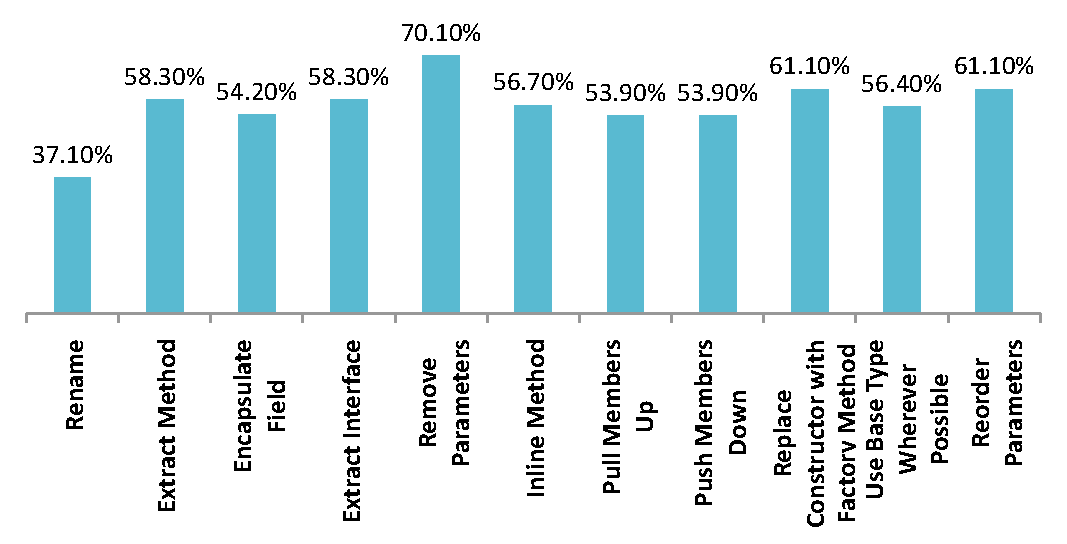
\includegraphics[width=0.55\textwidth]{images/manualRefactoring.pdf}
\centering
\caption{The percentage of survey participants who know individual refactoring types but do those refactorings manually.} 
\label{fig:manualRefactoring} 
\end{wrapfigure} 

\noindent{\bf Real-world enhancements are mostly done manually.} 
When we asked, {\it ``what percentage of your refactoring is done manually as opposed to using automated refactoring tools?''}, developers said they do 86\% of refactoring manually on average. Figure~\ref{fig:manualRefactoring} shows the percentages of developers who usually apply individual refactoring types manually despite the awareness of automated refactoring tool support. Vakilian et al.~\cite{Vakilian2012:usedisuse} and Murphy et al.~\cite{Murphy2006:JSD} also find that programmers do not use automated refactoring despite their awareness of the availability of automated refactorings. 
Our manual inspection of source code produced by 12 developers showed that, on average,
developers only used refactoring tools for 10\% of refactorings for which tools were
available~\cite{murphyHill10a}.

\noindent{\bf Real-world enhancements are error prone.} Wei{\ss}gerber and Diehl found that refactorings often occur together with other types of changes and that refactorings are followed by an increasing number of bugs~\cite{Weissgerber2006:refactor}. Our study of open source projects~\cite{Kim2011:refactorbug} found that the number of bug fixes increases after API refactorings. G{\"o}rg and Wei{\ss}gerber found errors caused by incomplete refactorings by relating API-level refactorings to the corresponding class hierarchy~\cite{Weissgerber2006:refactor}. Recent research found refactoring errors caused by tool-assisted refactorings as well. Daniel et al.~found dozens of bugs in the refactoring tools in popular IDEs~\cite{Brett2007:reftest}. We found that refactoring tools do a poor job of communicating errors~\cite{Murphy-Hill2009:refactor}. They also found that programmers frequently intersperse refactorings with other program changes\textemdash{\em floss} refactorings and these are not well supported by existing refactoring tools~\cite{Murphy-Hill2009:refactor}. This need for safe {floss} refactoring application is also confirmed by Kim et al.'s study~\cite{Kim2011:refactorbug}\textemdash refactoring often overlap with bug fixes, {\em behavior correcting} transformations. {\em Program metamorphosis} relaxes behavior-preservation checks to safely support floss refactorings~\cite{Reichenbach2009:pm}.

When we asked developers, {\it ``based on your experience, what are the risks involved in refactorings?''}, they reported regression bugs, code churn, merge conflicts, time taken from other tasks, the difficulty of doing code reviews after refactoring, and the risk of over-engineering~\cite{Kim2012:fieldrefactoring}. 77\% think that refactoring comes with a risk of introducing subtle bugs and functionality regression~\cite{Kim2012:fieldrefactoring}.

\noindent{\bf Real-world enhancements do not fit developers' workflow.} 
As we noted above, even when developers are aware of refactoring tools, they rarely use them.  In a study of refactoring tool use, we gave developers specific examples of when they did not use refactoring tools, but could have~\cite{murphyHill10a}.  We then asked them why they did not use the tools.  One reason was that developers started a refactoring manually, but only partway through realized that the change was a refactoring that the IDE offered\textemdash by then, it was too late.  Another complaint was that refactoring tools disrupted their workflow, forcing them to use a tool when they wanted to focus on code.  Other restructuring tools, such as code generation tools, likely suffer from the same issue.  These problems illustrate how traditional refactoring tools do not fit into the development workflow.

\subsubsection{Code Smells Detection} 

Fowler~\cite{fowler:refactor99} describes the concept of {\em bad smell} as a heuristic for identifying redesign and refactoring opportunities. Example bad smells include code clone and feature envy. Garcia et al.~\cite{garcia:csmr09} proposed several architecture-level bad smells. To automate the identification of bad smells, Moha et al.~\cite{moha:fase08} presented the Decor tool and domain specific language (DSL) to automate the construction of design defect detection algorithms.  Several other techniques ~\cite{tsantalis:csmr09, tsantalis:tse09, tsantalis:csmr08} automatically identify bad smells that indicate needs of refactorings. For example, Tsantalis and Chatzigeorgiou's technique~\cite{tsantalis:csmr09} identifies {\em extract method} refactoring opportunities using static slicing. Detection of some specific bad smells such as code duplication has also been extensively researched. Higo et al.~\cite{higo:profes04} proposed the Aries tool to identify possible refactoring candidates based on the number of assigned variables, the number of referred variables, and dispersion in the class hierarchy. A refactoring can be suggested if the metrics for the clones satisfy certain predefined values. Komondoor's technique~\cite{Komondoor2003} extracts non-contiguous lines of clones into a procedure that can then be refactored by applying an {\em extract method} refactoring. Koni-N'Sapu~\cite{KONI01} provides refactoring suggestions based on the location of clones with respect to a system's class hierarchy. Balazinska et al.~\cite{Balazinska2000} suggest clone refactoring opportunities based on the differences between the cloned methods and the context of attributes, methods, and classes containing clones. {\it Breakaway} \cite{Cottrell2007} automatically identifies detailed structural correspondences between two abstract syntax trees to help programmers generalize two pieces of similar code. Tsantalis and Chatzigeorgiou's technique~\cite{Tsantalis2009:extractmethod,Tsantalis2008:jdeodorant} identifies {\em extract method} refactoring opportunities using static slicing. Our work is different from these refactoring opportunity identification techniques in that it uses clone {\em evolution history} to predict how long clones are likely to survive in a system. 

Gueheneuc et al.~detect inter-class design defects~\cite{Gueheneuc2001:designdefect} and Marinescu identifies design flaws using software metrics~\cite{Marinescu2004:designflaw}. Izurieta and Bieman detect accumulation of non design-pattern related code~\cite{Izurieta2007:grime}. Guo et al.~define domain-specific code smells~\cite{Guo2010:smell} and investigate the consequence of technical debt~\cite{Guo2011:td}.

Clio~\cite{Wong2011:cleo} detects modularity violations based on the assumptions that multiple types of bad smells are instances of modularity violations that can be uniformly detected by reasoning about modularity hierarchy in conjunction with change locations.  They define {\em modularity violations} as recurring discrepancies between which modules should change together and which modules actually change together according to version histories. For example, when code clones change frequently together, Clio will detect this problem because the co-change pattern deviate from the designed modular structure. Second, by taking version histories as input, Clio detects violations that happened most recently and frequently, instead of bad smells detected in a single version without regard to the program's evolution context. Similar to Clio, Ratzinger et al.~\cite{ratzinger:msr05} also detect bad smells by examining change couplings but their approach leaves it to developers to identify design violations from visualization of change coupling. On the other hand, Clio locates violations by comparing change coupling with structural coupling. The detected violations thus either reflect the problem in the original design or introduced in the subsequent modification requests.

Related to the problem of code smells detection, various approaches have been proposed to automatically suggest refactoring opportunities based on program context or version history~\cite{Balazinska2000:ACA,Kataoka2001:ASP,Higo2008:metricrefactoring,Tsantalis2011:rankRefactoring,Wang2014:recommendClones,Meng2015:ARO}. Specifically, Kataoka et al.~developed Daikon to infer program invariants at runtime, and thus to suggest candidate refactorings~\cite{Kataoka2001:ASP}. For instance, if Daikon observes that one parameter of a method is always constant, it then suggests a \emph{removeParameter} refactoring. Balazinska et al.~used a clone detection tool to identify duplicated code and to suggest clone removal refactorings~\cite{Balazinska2000:ACA}. Tsantalis et al.~ranked clones that have been repetitively or simultaneously changed in the past to suggest refactorings~\cite{Tsantalis2011:rankRefactoring}. Wang et al.~extracted features from code to reflect program context, code smell, and evolution history, and then used a machine learning technique to rank clones for refactorings~\cite{Wang2014:recommendClones}.

\subsubsection{Checking the Behavior-Preserving Property of Refactorings}Opdyke suggested to ensure such behavior preservation by specifying \emph{refactoring preconditions}~\cite{Opdyke1992:ROF}. For instance, when conducting an \emph{create\_method\_function} refactoring, before inserting a member function $F$ to a class $C$, developers should specify and check for five preconditions, as shown in Figure~\ref{fig:preconditions}. If any precondition is not satisfied, the refactoring should not be applied to the program.

\begin{figure}[!htb]
\centering
\scalebox{0.55}{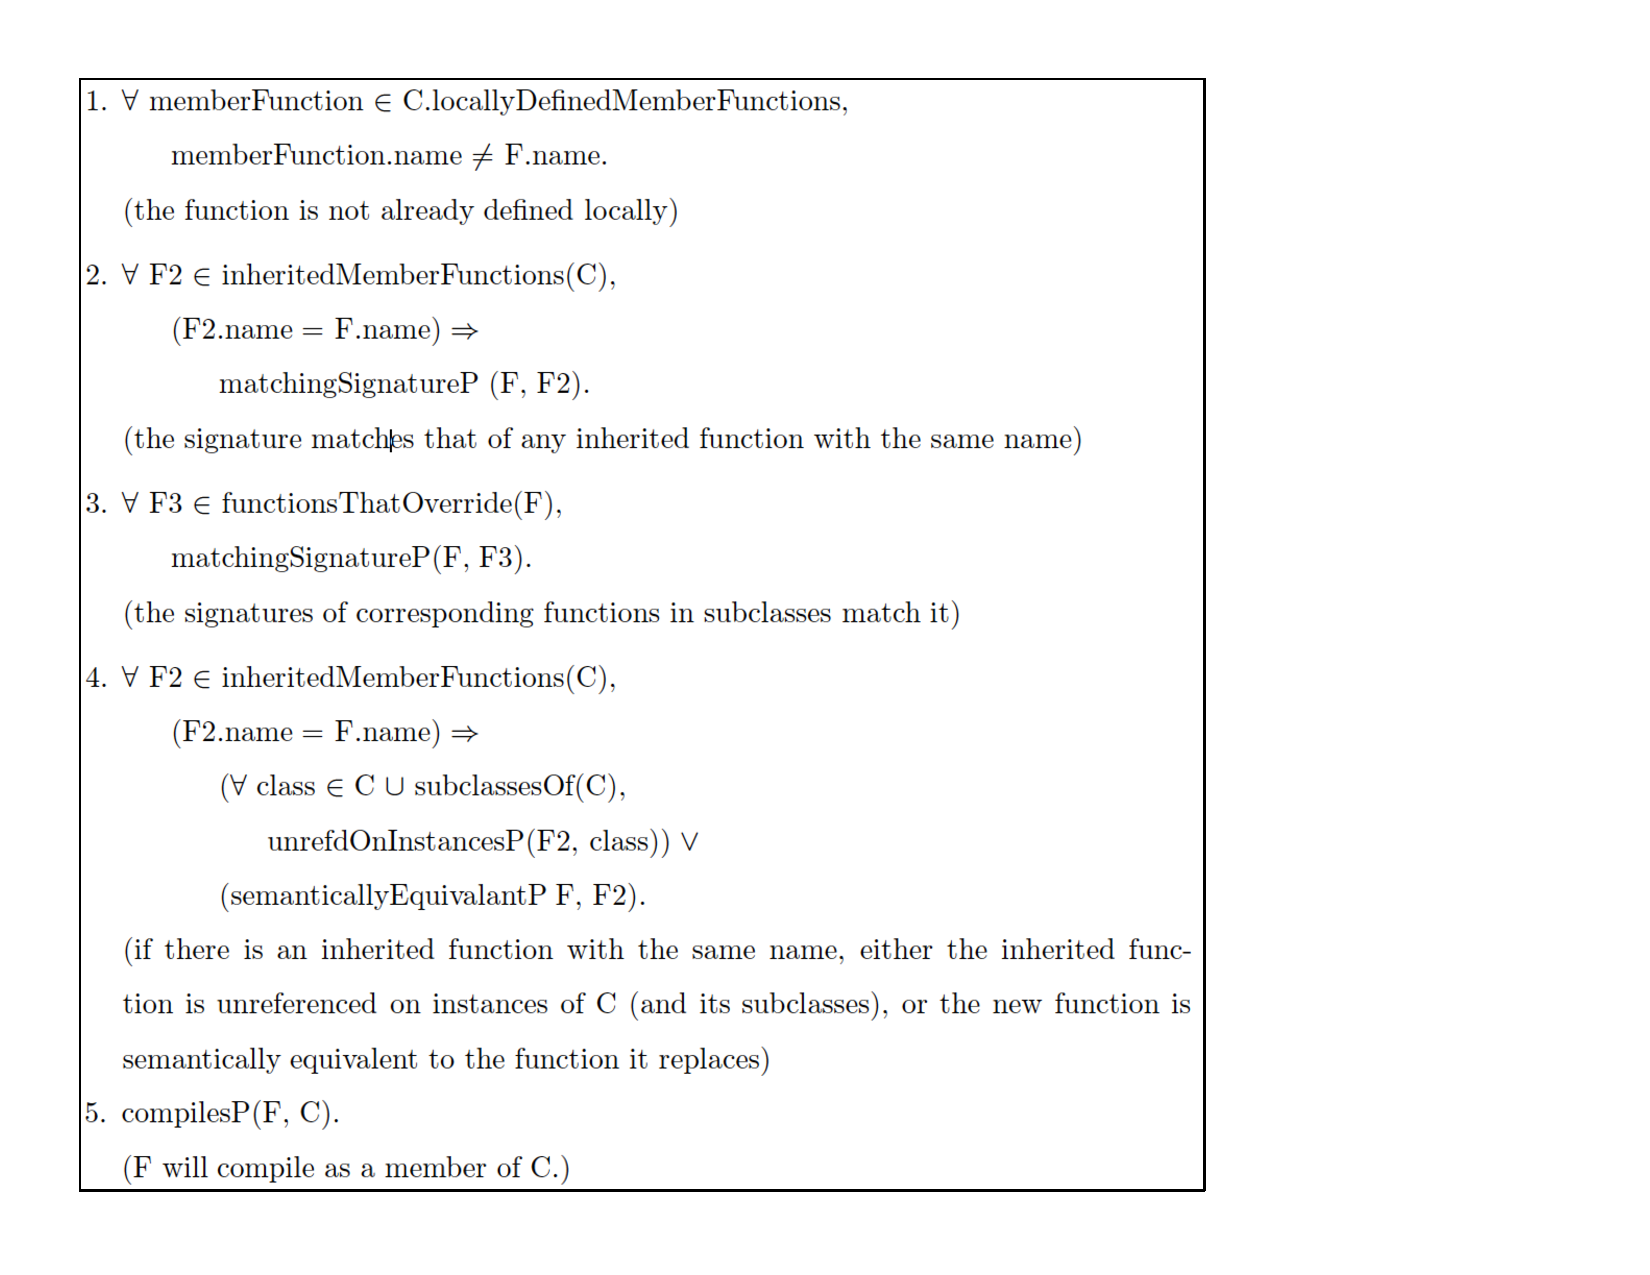
\includegraphics{images/preconditions.pdf}}
\caption{Preconditions for \emph{create\_method\_function} refactoring~\cite{Opdyke1992:ROF}}
\label{fig:preconditions}
\end{figure}
\subsection{Automatic Change Application}
\label{sec:automatic}


\begin{figure}[ht]
 \centering
 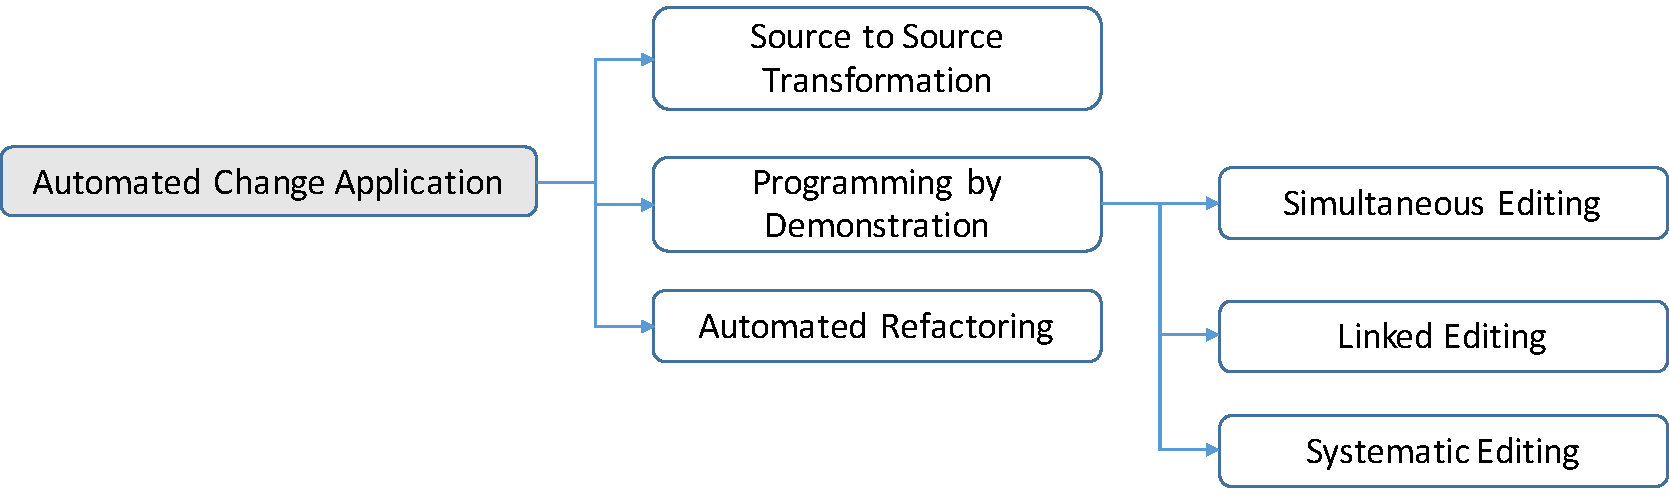
\includegraphics[width=0.95\textwidth]{images/AutomatedChange.pdf}
 \caption{Automated Change Application and Related Research Topics} 
 \label{fig:automaticapplication} 
\end{figure}



Regardless of change types, various approaches are proposed to automatically suggest program changes to developers or reduce the manual effort of updating software. In this section, we discuss automated change application techniques including source-to-source program transformation, Programming by Demonstration (PbD), simultaneous editing, and systematic editing.

\subsubsection{Source Transformation and Languages and Tools} 

Source transformation tools allow programmers to author their change intent in a formal syntax and automatically update a program using the change script. Most source transformation tools automate repetitive and error-prone program updates. The most ubiquitous and the least sophisticated approach to program transformation is text substitution. More sophisticated systems use program structure information. For example, A* \cite{Ladd1995} and TAWK \cite{Griswold1996} expose syntax trees and primitive data structures. Stratego/XT\cite{Visser2004} is based on algebraic data types and term pattern matching. These tools are difficult to use as they require programmers to understand low-level program representations. TXL \cite{Cordy2006} attempts to hide these low-level details by using an extended syntax of the underlying programming language. Boshernitsan et al.'s iXJ \cite{Boshernitsan2007} enables programmers to perform systematic code transformations easily by providing a visual language and a tool for describing and prototyping source transformations. Their user study shows that iXj's visual language is aligned with programmers' mental model of code changing tasks. Erwig and Ren \cite{Erwig2002} designed a rule-based language to express systematic updates in Haskell. Coccinelle \cite{Padioleau2008} allows programmers to safely apply crosscutting updates to Linux device drivers. 

While these tools focus on applying systematic changes to a program, our approach focuses on recovering systematic changes from two versions. 
Despite the significant difference in their goals, both approaches' change-representations capture systematic changes concisely and explicitly. In theory, one can build a program differencing tool using a source transformation tool's change-representation by (1) automatically enumerating potential transformations, (2) applying the transformations to the old program version, and (3) checking whether the updated program is the same as the new program version. 
However, the change-representation's granularity and expressive power will affect its use for high-level reasoning of program differences. 

\paragraph{\textbf{TXL.}} 

TXL is a programming language and rapid prototyping system specifically designed to support structural source transformation. TXL's source transformation paradigm consists of parsing the input text into a structure tree, transforming the tree to create a new structure tree, and unparsing the new tree to a new output text. Source text structures to be transformed are described using an unrestricted ambiguous context free grammar in extended Backus-Nauer (BNF) form. Source transformations are described by example, using a set of context sensitive structural transformation rules from which an application strategy is automatically inferred. 

Each transformation rule specifies a {\em target type} to be transformed, a {\em pattern} (an example of the particular instance of the type that we are interested in replacing), and a {\em replacement} (an example of the result we want when we find such an instance). In particular, the pattern is an actual source text example expressed in terms of tokens (terminal symbols) and variables (non-terminal types). When the pattern is matched, variable names are bound to the corresponding instances of their types in the match. Transformation rules can be composed like function compositions.  Figure \ref{txl_rule} shows an example TXL rule that replaces \codefont{(1+1)} expressions with \codefont{2}. 

\begin{figure} 
\codefont{rule addOnePlusOne} \% target structure \newline
\indent \codefont{replace [expression]}  \% pattern to search for \newline
\indent \indent \codefont{1+1} \newline
\indent \codefont{by } 
\indent \indent \codefont{2} \newline \% replacement to make \newline
\codefont{end rule} \newline
\caption{Example TXL rule} 
\label{txl_rule} 
\end{figure} 

TXL's transformation rules in general require programmers to obtain the knowledge of syntax trees. Though it is well suited for systematic changes at an expression level, it is less suited for expressing systematic changes at a higher abstraction level such as moving a set of classes from one package to another package. In addition, as our change-rules abstract a program at the level of code elements and structural dependencies, our approach finds systematic change patterns even when the constituent transformations are not exactly the same; For example, adding call dependencies to a particular method is grouped as a single rule even if the input parameters in the call invocation statements vary. 

\paragraph{\textbf{iXj.}} 
iXj's pattern language consists of a {\em selection pattern} and a {\em transformation action}. A selection pattern is similar to our rules' antecedent, and a transformation action is similar to our rules' consequent. Similar to our API change-rules, iXj's transformation language allows grouping of code elements using a wild-card symbol \codefont{*}. Figure \ref{ixj_example} shows an example selection pattern and a transformation pattern. 

\begin{figure} 
Selection pattern: \codefont{* expression instance of java.util.Vector (:obj).removeElement(:method)(* expressions(:args))} \\
\it{Match calls to the {removeElement()} method where the {obj} expression is a subtype of {java.util.Vector}.} 

Transformation action: \codefont{\$obj\$.remove(\$obj\$.indexOf(\$args\$))} \\
\it{Replace these calls with with calls to the {remove()} method whose argument is the index of an element to remove.} 

\caption{Example iXj transformation} 
\label{ixj_example} 
\end{figure} 


To reduce the burden of learning the iXj pattern language syntax, iXj's visual editor scaffolds this process through from-example construction and iterative refinement; When a programmer selects an example code fragment to change, iXj automatically generates an initial pattern from the code selection and visualizes all code fragments matched by the initial pattern. The initial pattern is presented in a pattern editor, and a programmer can modify it interactively and see the corresponding matches in the editor. A programmer may edit the transformation action and see the preview of program updates interactively. 

Similar to TXL, iXj's transformation language works at the level of syntax tree nodes, mostly at an expression level. Thus, it is not effective for expressing higher-level transformation such as moving a set of related classes from one package to another package. Its transformation actions are more expressive than our change-rules in that they support free-form text edits.

The above source transformation languages and tools are appropriate in situations where developers are willing to plan changes in advance and to learn a transformation language to precisely encode those changes.

\subsubsection{Programming by Demonstration.} 
PbDis also called Programming by Example (PbE). It is an end-user development technique for teaching a computer or a robot new behaviors by demonstrating the task to transfer directly instead of manually programming the task.
Approaches were built to generate programs based on the text-editing actions demonstrated or text change examples provided by users~\cite{Nix1984,WiM1993,LaH1995,LWD2001}. For instance, 
TELS records editing actions such as search-and-replace, and generalizes them into a program that transforms input to output~\cite{WiM1993}. It leverages heuristics to match actions against each other to detect any loop in the user-demonstrated program. 
Similarly, SMARTedit~\cite{LWD2001} automates repetitive text-editing tasks by learning programs to perform them using techniques drawn from machine learning. SMARTedit represents a text-editing program as a series of functions that alter the state of the text editor (i.e., the contents of the file, or the cursor position). Like macro recording systems, SMARTedit learns the program by observing a user performing her task. However, unlike macro recorders, SMARTedit examines the context in which the user's actions are performed and learns programs that work correctly in new contexts. 

\subsubsection{Simultaneous Editing.}
Simultaneous editing repetitively applies source code changes that are interactively demonstrated by users~\cite{MiM2001}. When users apply their edits in one program context, the tool replicates the \emph{exact lexical} edits to other code fragments, or transforms code accordingly. For instance, Linked Editing requires users to first specify the similar code snippets which they want to modify in the same way~\cite{TBG2004}. As users interactively edit one of these snippets, Linked Editing simultaneously applies the identical edits to other snippets. 
CloneTracker takes the output of a clone detector as input and creates a descriptor for each clone~\cite{DuR2007}. With such descriptors, CloneTracker tracks clones across program versions and identifies any modification to those clones. 
Similar to Linked Editing, CloneTracker also echoes edits in one clone to other counterparts upon a developer's request. 
Clever is another clone management system that tracks code clone groups and detects any inconsistent change applied to clones within the same group~\cite{NNP2009}. If a clone misses the updates applied to the other clones in the same group, Clever automatically suggests the missing update to that clone.

\subsubsection{Systematic Editing.} 
Systematic editing is the process of applying similar, but not necessarily identical, program changes to multiple code locations. 
High-level changes are often systematic\textemdash consisting of related transformations at a code level. The same insight arises from numerous other research efforts, primarily within the domain of refactorings and crosscutting concerns. {\em Refactoring} is the process of changing a software system that does not alter the external behavior of the code, yet improves the internal structure~\cite{Fowler2000, Griswold1991, Mens2004, Opdyke1992}. Refactorings often consist of one or more elementary transformations, such as ``moving the \codefont{print} method in {\bf \em each} \codefont{Document} subclass'' or ``introduce {\bf \em three} abstract \codefont{visit*} methods.'' {\em Crosscutting concerns} represent secondary design decisions\textemdash e.g., performance, error handling, and synchronization\textemdash that are generally scattered throughout a program \cite{Kiczales1997, Tarr1999}. Modifications to these design decisions involve similar changes to every occurrence of the design decision. To cope with evolution of crosscutting concerns, AspectJ provides language constructs that allow these concerns to be updated in a modular fashion \cite{Kiczales2001}. Several techniques~\cite{Breu2006, Dagenais2007} locate and document crosscutting concerns based on similarities in a program's dependency structure, naming conventions, formatting styles, and ordering of code in a file \cite{Griswold2001}. 

%Prior work shows that programmers apply systematic edits to either add features, fix bugs, or refactor code~\cite{Kim:2005,Kim:2009,Nguyen:2010}. 
Manually applying systematic edits is tedious and error-prone. 
%for two reasons. 
%First, developers may forget to apply systematic edits to all program contexts where the edits are needed, committing errors of omission. Second, developers may apply edits inconsistently and thus introduce new bugs. 
%To improve programmer productivity and software quality, 
Several approaches~\cite{MKM2011,MKM2013,Rolim:2017} have been proposed to infer the general program transformation from one or more code change examples provided by developers, and then apply the transformation to other program contexts in need of similar changes. Specifically, LASE requires developers to provide multiple similarly changed Java methods (at least two)~\cite{MKM2013}. By extracting the commonality between demonstrated changes and abstracting the changes in terms of identifier usage and control- or data-dependency constraints in edit contexts, LASE creates a general program transformation, which can both detect code locations that should be changed similarly, and suggest customized code changes for each candidate location.

\subsubsection{Suggesting Edit Location.}


\paragraph*{Suggesting edit locations.}
LibSync helps client applications migrate library API usages by learning migration patterns~\cite{Nguyen2010:libsync} with respect to a partial AST with containment and data dependences. Though it suggests what code locations to examine and shows example API updates, it is \emph{unable} to transform code.  Furthermore, its flexibility is limited by its inability to abstract variable, method, and type names.

FixWizard identifies code clones based on object usage and interactions, recognizes recurring bug-fixes to the clones, and suggests a location and example edit~\cite{Nguyen2010:fixwizard}. FixWizard identifies edit locations automatically only in pre-identified clones.  It does {\em not generate syntactic edits}, nor does it support abstraction of variables, methods, and types. These limitations leave programmers with the burden of manually editing the suggested fix-location, which is error-prone and tedious.

\subsection{Other Studies of Software Evolution} 
Kemerer and Slaughter \cite{Kemerer1999} manually coded over 25000 change logs to classify each change event to 6 types of corrective, 6 types of adaptive, and 6 types of perfective changes. Their analysis used phase mapping and gamma sequence analysis methods originally developed in social psychology to identify and understand the phases of software evolution. 

Eick et al. \cite{Eick2001} developed a process for analyzing the change history of the code, which is assumed to reside in a version management system, calculating code-decay indices, and predicting the fault potential and change effort through regression analysis. The objective of this research is to support project management so that code decay is delayed. 

Hassan and Holt \cite{Hassan2003} studied the chaos of software systems in terms of information entropy\textemdash the amount of uncertainty related to software products. Intuitively, in the context of software evolution, if a software system is being modified across all its modules, it has high entropy, and the software maintainers will have a hard time keeping track of all the changes. Their work relies on maintenance documentation to keep track of software modifications in order to compute information entropy of files that evolved over a period of time. 

The major drawback of this line of research is that it requires developers' comments recorded in the version management system. In most real-world software projects, comments are inconsistent in their detail and they often do not even exist. 

\subsection{Visualization of Software Evolution} 
There are several visualization techniques that focus on software evolution, in particular, changes in software-process statistics, source code metrics, static dependence graphs, {\it diff}-based deltas and their derivatives, etc. 

% ball 1996 - software visualization in the large
Ball et al. \cite{Ball1996} developed the one of the first systems that \cite{Ball1996} explored visualizing software evolution data, in particular, the age of individual code lines as a color. Their work also visualizes program differences between two versions, which are calculated using {\it diff}.

%Holt and Pak 1996 
Holt and Pak \cite{Holt1996} visualized structural changes between two program versions by explicitly modeling code elements and their structural dependencies. Their visualization focuses on which structural dependencies are common, which dependencies are new, and which dependencies are deleted between two versions at the subsystem level. 

% ball 1997 - if version control system could talk. 

%eick 2002
Eick et al.~\cite{Eick2002} developed a number of views (matrix, cityscape, bar and pie charts, data sheets, and network) that facilitate rapid exploration of high-level structure in software evolution data and also serve as a powerful visual interface to the data details as needed. These visualization tools explicitly model logical software changes as their visualization is built upon proprietary evolution history data, where a set of related program deltas are grouped to a logical software change called a modification request (MR) and its change type is manually written by developers as an adaptive, corrective, or perfective change. 

% pingzger 2005 -RelVis
Pinzger et al.'s RelVis approach \cite{Pinzger2005} condenses multi-dimensional software evolution metric data into two graphs. The first graph visualizes modules and their metrics over time. The second graph visualizes relationships between source code modules. In both graphs, the evolution of metrics is visualized using a Kiviat diagram where annual rings indicate metric values for each release.

% Lanza 2003 
Lanza and Ducasse's Polymetric views \cite{Lanza2003} is a lightweight software visualization technique enriched with software metrics information. Polymetric views help to understand the structure and detect problems of a software system in the initial phases of a reverse engineering process by combining software visualization and software metrics. Lanza applied this general visualization technique to metric values over multiple program versions, and named this view an evolution matrix \cite{Lanza2001}. This view is instantiated at two granularity levels (a system level or a class level) and can help programmers understand how the system size grows, when and where classes are added or deleted, etc. 

%Girba 2004
Girba et al. \cite{Girba2004} introduced the {\it Yesterday's Weather} metric that can further condense historical change patterns at a class granularity. This metric is designed to help a programmer identify a candidate for further reverse engineering based on the observation that classes that changed most in the recent past are likely to undergo important changes in the near future. 
 
%Rysselberge 2004
Rysselberghe et al. \cite{Rysselberghe2004a} proposed a dot plot visualization of change data extracted from a version control system to identify unstable components, coherent entities, productivity fluctuations, etc.  

These visualization techniques assume a substantial interpretation effort on behalf of their users and do not scale well. They become unreadable for a long evolution history of large systems with numerous components. In addition, many of these techniques are inherently limited by the source of history data\textemdash most version control systems consider a software system as a set of files containing lines of texts and consequently they report changes at the lexical level and are unaware of the high-level logical structural changes of the software system. 

\section{An Organized Tour of Seminal Papers: II. Inspecting Changes}
\label{sec:inspect}

\begin{figure}[ht]
 \centering
 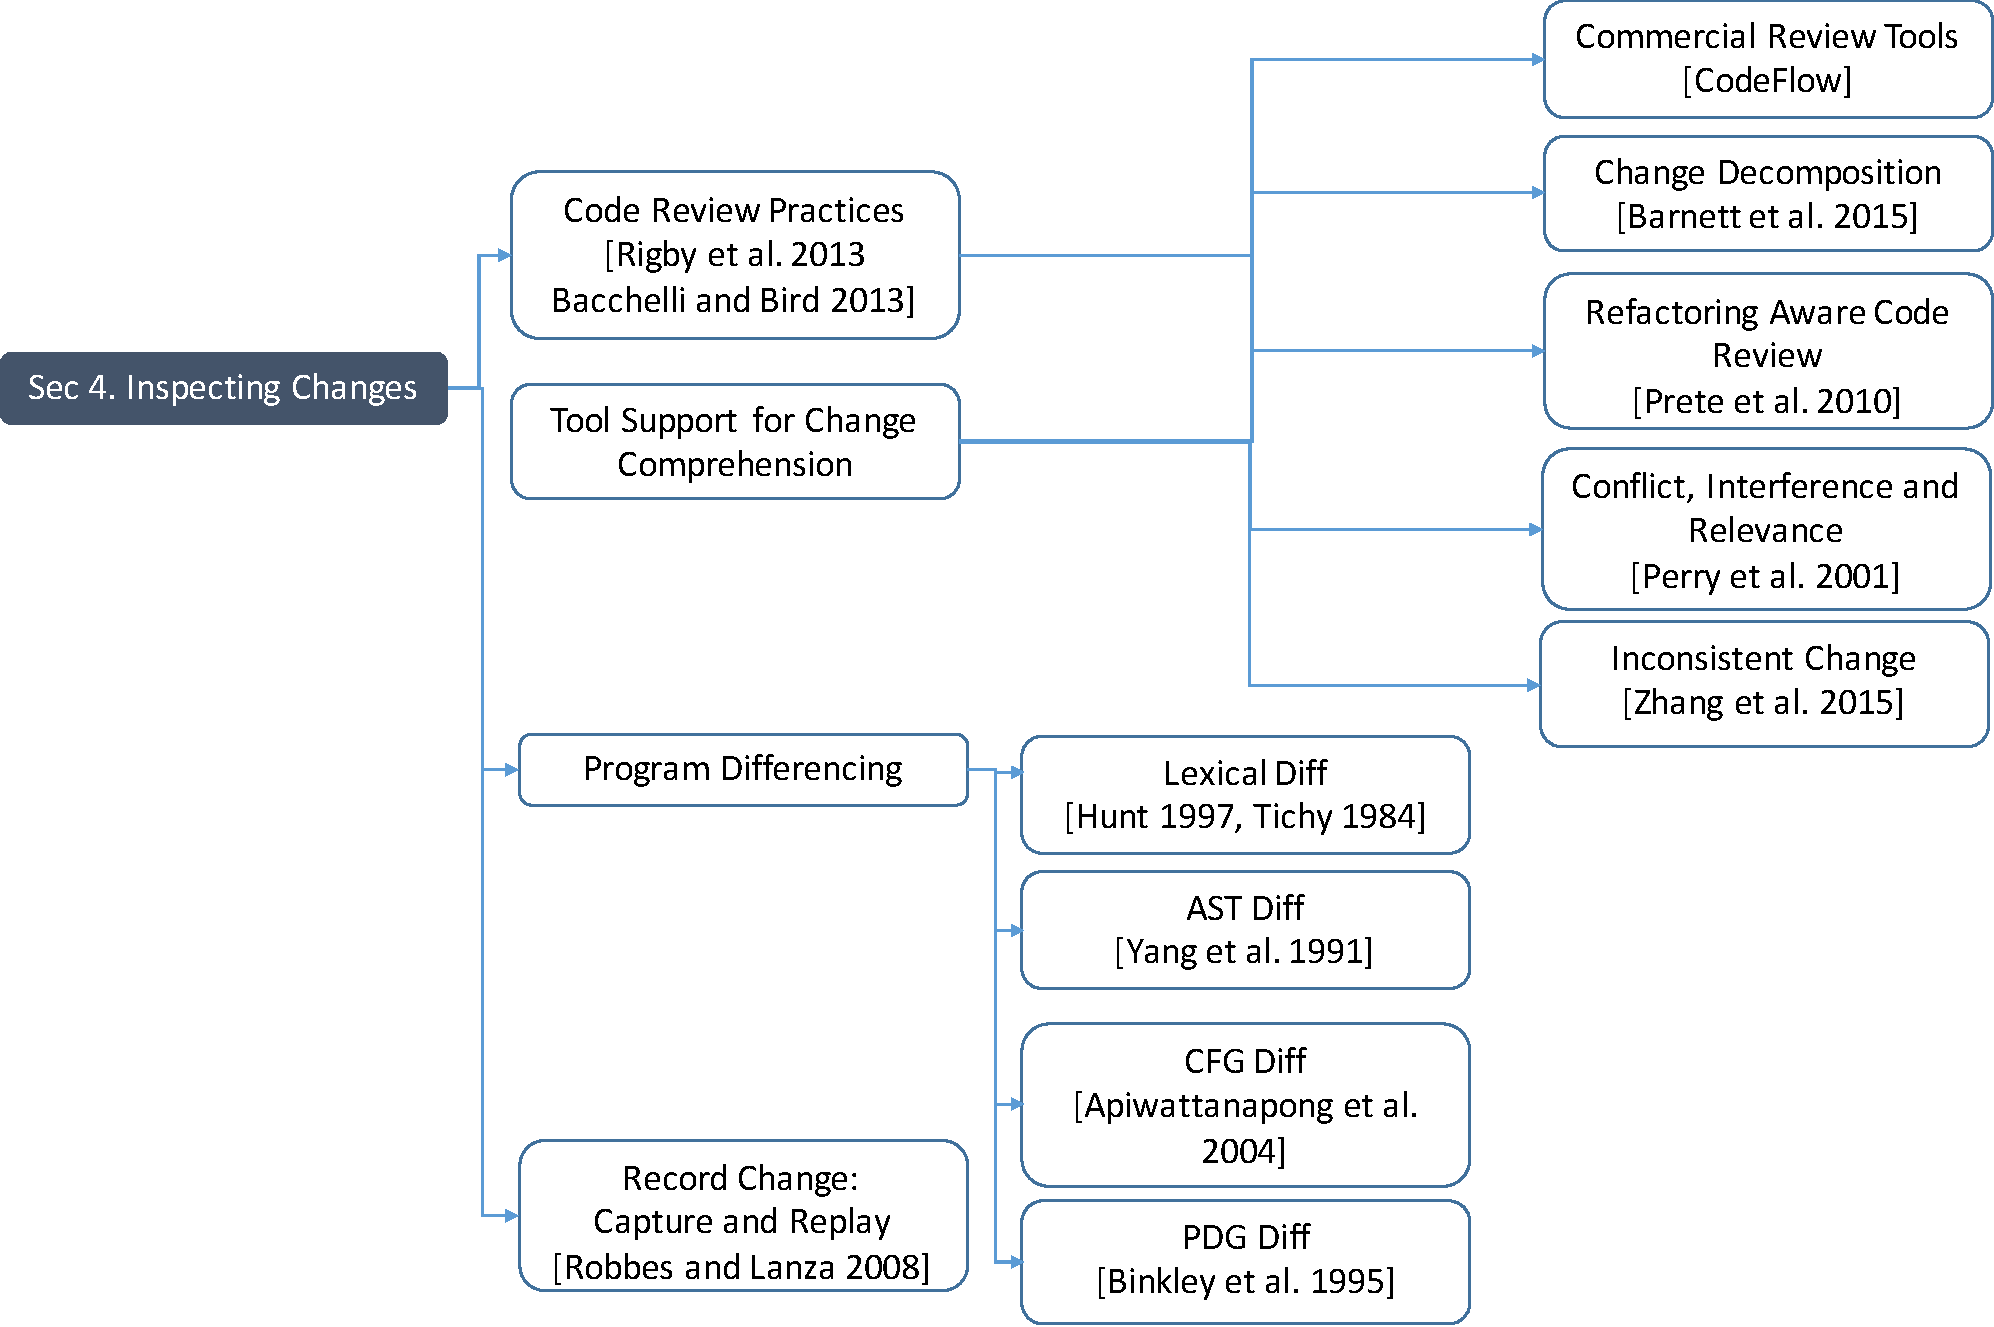
\includegraphics[width=0.95\textwidth]{images/ChangeInspection.pdf}
 \caption{Change Inspection and Related Research Topics} 
 \label{fig:changeinspection} 
\end{figure}

\subsection{Code Review Practices}
To improve the correctness and quality of software systems, developers often perform {\em code reviews} to manually examine program changes made to software systems. Michael Fagan from IBM first introduced ``code inspections'', the original name, in a seminal paper in 1976~\cite{fagan2001design}. Code inspections are performed at the end of major software development phases, with the aim of finding overlooked defects before moving to the next phase. Software artifacts are circulated a few days in advance and then reviewed and discussed in a series of meetings. The meetings include the author of an artifact, other developers to assess the artifact, and a meeting chair to moderate the discussion, and a secretary to record the discussion. Over the years, code inspections have been proven a valuable method to improve the software quality. However, the cumbersome and time-consuming nature of this process hinders its universal adoption in practice~\cite{johnson1998reengineering}. 

\begin{figure}[ht]
 \centering
 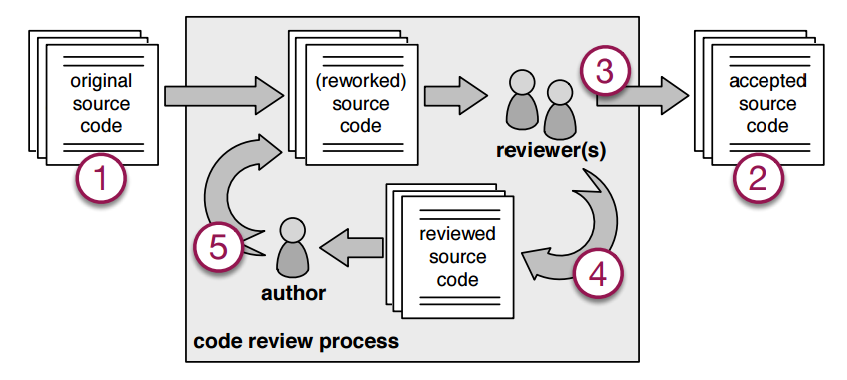
\includegraphics[width=0.75\textwidth]{images/review-process.png}
 \caption{Modern Code Review Process~\cite{beller2014modern}}
 \label{fig:review-process}
\end{figure}

To avoid the inefficiencies in code inspections, most open-source and industrial projects adopt a lightweight, flexible code review process, which we refer to as {\em modern code reviews}. Figure~\ref{fig:review-process} shows the workflow of modern code reviews. The {\em author} first submits the {\em original source code} for review. The {\em reviewers} then decide whether the submitted code meets the quality acceptance criteria. If not, reviewers can annotate the source code with review comments and send back the {\em reviewed source code}. The author then revises the code to address reviewers' comments and send it back for further reviews. This process continues till all reviewers accept the revised code.

In contrast to formal code inspections (Fagan style), modern code reviews occur more regularly and informally on small yet complete program changes. 
%Mockus et al.~studied the defects in Apache bug database and found the Apache project has a defect density comparable to proprietary software~\cite{mockus2000case}. They found that this was accomplished without a policy requiring substantial code reviews before a release. They comment that this result ``may indicate that fewer defects are injected into the code, or that other defect-finding activities such as inspections are conducted more frequently or more effectively''. 
Rigby et al.~conducted the first case study about modern code review practices in an open-source software (OSS), Apache HTTP server, using archived code review records in email discussions and version control histories~\cite{rigby2008open}. They described modern code reviews as ``early, frequent reviews of small, independent, complete contributions conducted asynchronously by a potentially large, but actually small, group of self-selected experts.'' As code reviews are practiced in software projects with different settings, cultures, and policies, Rigby and Bird further investigated code review practices in a diverse set of open-source and industrial projects~\cite{rigby2013convergent}. Despite differences among projects, they found that many characteristics of modern code reviews have independently converged to similar values, indicating general principles of modern code review practices. We summarize these convergent code review practices as following.

{\bf Modern code reviews occur early, quickly, and frequently.} Traditional code inspections happen after finishing a major software component and often last several weeks. In contrast, modern code reviews happen more frequently and quickly around the time when program changes are committed. Rigby et al.~found that the Apache project has review intervals between a few hours to a day. Rigby and Bird also observed that most reviews are picked up within a few hours among all projects, indicating that reviewers are regularly watching and performing code reviews~\cite{rigby2013convergent}.

{\bf Modern code reviews often examine small program changes.} In the OSS project studied by Rigby et al., the median change varies from 11 to 32 changed lines. The median change size in industrial projects is larger, e.g, 44 lines in Android, 78 lines in Chrome, but still much smaller than code inspections, e.g., 263 lines in Lucent. Such small changes also facilitate developers to constantly review changes and thus keep up-to-date with the activities of their peers. 

{\bf Modern code reviews are conducted by a small group of self-selected reviewers.} 
%Traditional code inspections require a designated inspection team where team members have particular roles.
In OSS projects, no reviews are assigned and developers can select the changes of interest to review. Program changes and review discussions are broadcast to a large group of stakeholders but only a small number of developers periodically participate into code reviews. In industrial projects, reviews are assigned in a mixed manner---the author adds a group of reviewer candidates and individuals from the group then select changes to review based on their interest and expertise. Rigby and Bird found that two reviewers find a optimal number of defects~\cite{rigby2013convergent}.

{\bf Modern code reviews are often tool-based.} There is a clear trend towards utilizing review tools to support review tasks and communication. Back in 2008, Rigby et al.~reported that code reviews in OSS projects were often email-based due to a lack of tool support. In 2013, Rigby and Bird found that some OSS projects and all industrial projects they studied used a review tool. More recently, popular OSS hosts such as GitHub and BitBucket have integrated lightweight review tools to assign reviewers, enter comments, and record discussions. Compared with email-based reviews and traditional inspections, tool-based reviews provide the benefits of traceability and can record implicit measures. The rise in adoption of review tools provides an indicator of success.

Although the initial purpose of code review is to find defects, recent studies find that the practices and actual outcomes are less about finding defects than expected. Bacchelli and Bird studied hundreds of review comments at Microsoft and found that only a small portion of review comments were related to defects, which were mainly about small, low-level logical issues~\cite{bacchelli2013expectations}. Rather, code review provides a spectrum of benefits to software teams, such as knowledge transfer, team awareness, and improved solutions with better practices and readability. 

\subsubsection{Commercial Code Review Tools} 

There is a proliferation of review tools, e.g., Phabricator,\footnote{\url{http://phabricator.org}} Gerrit,\footnote{\url{http://code.google.com/p/gerrit/}} CodeFlow,\footnote{\url{http://visualstudioextensions.vlasovstudio.com/2012/01/06/codeflow-code-review-tool-for-visual-studio/}} Crucible,\footnote{\url{https://www.atlassian.com/software/crucible}} and Review Board.\footnote{\url{https://www.reviewboard.org/}} We will illustrate CodeFlow, a collaborative code review tool at Microsoft. Other review tools share similar functionality as CodeFlow.

\begin{figure}[ht]
 \centering
 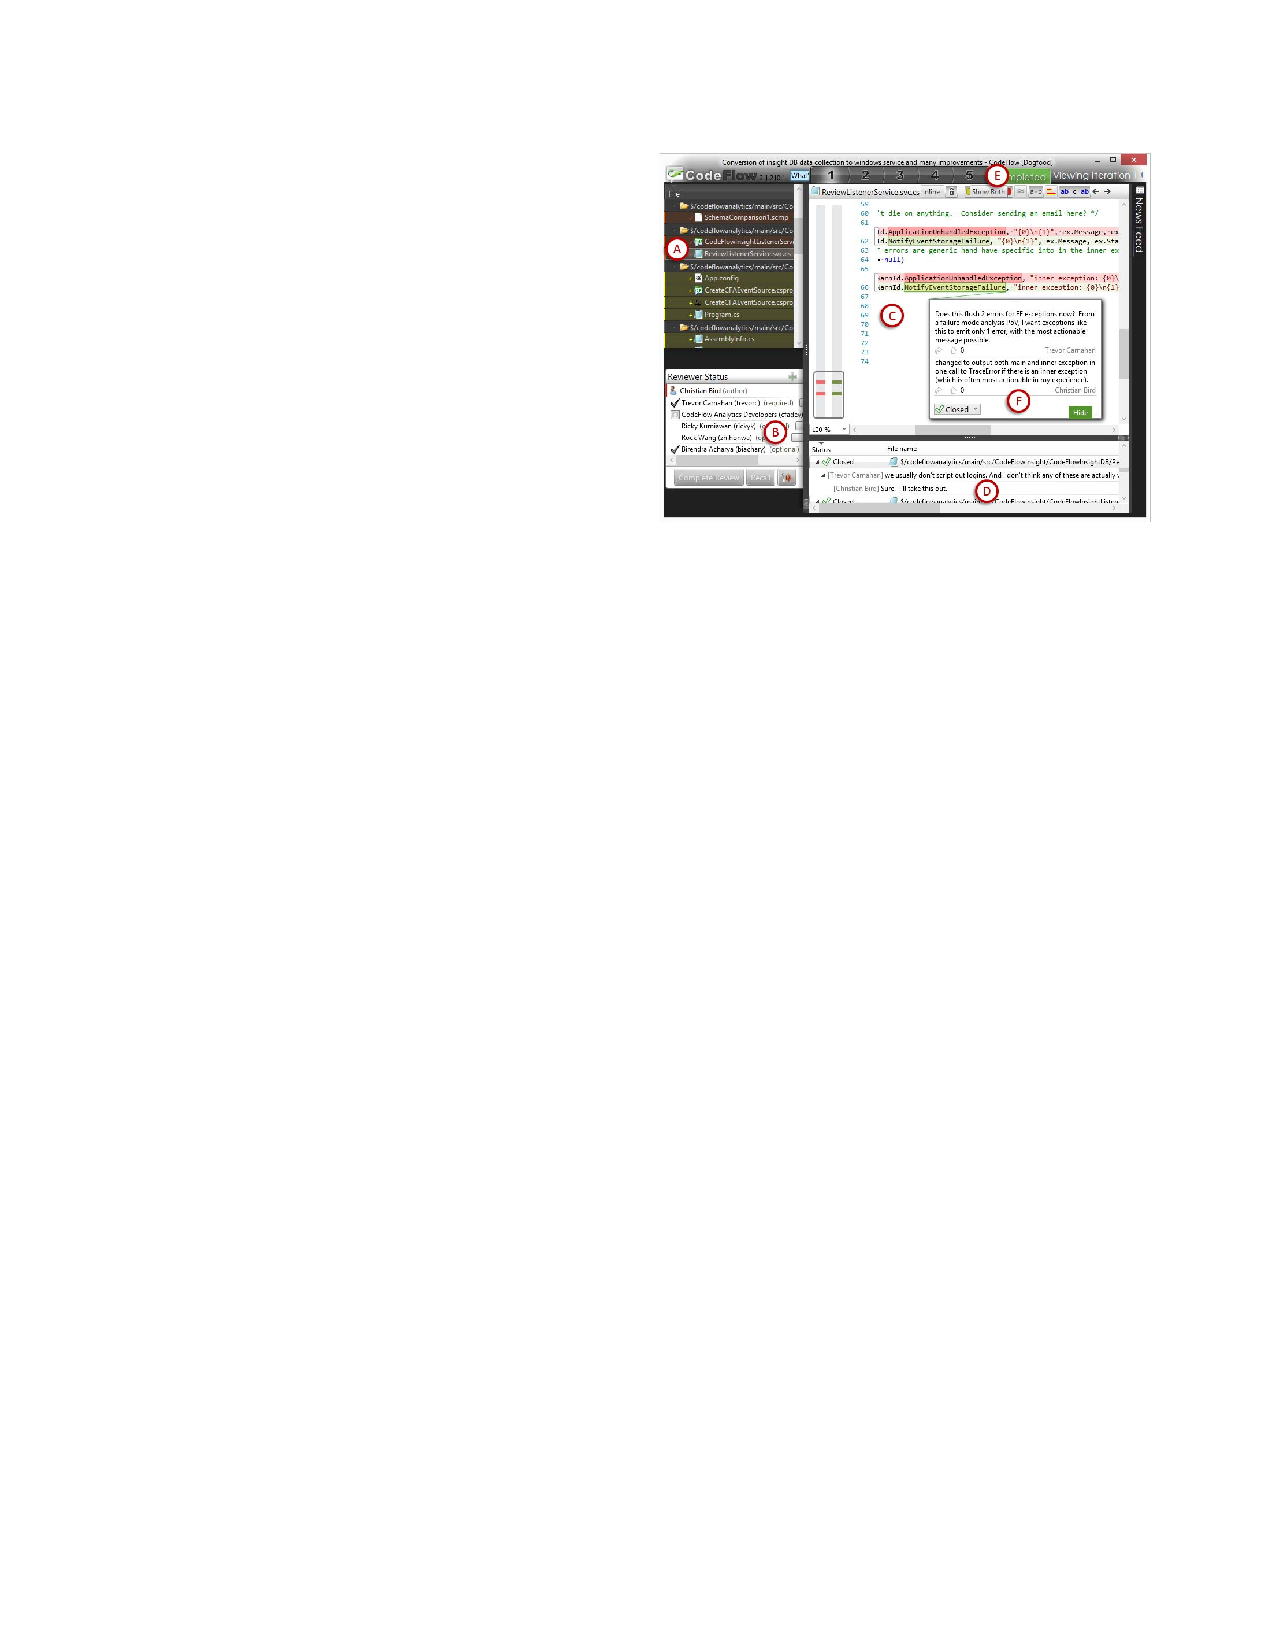
\includegraphics[width=0.75\textwidth]{images/codeflow.pdf}
 \caption{Example of Code Review using CodeFlow~\cite{bosu2015characteristics}}
 \label{fig:codeflow}
\end{figure}

To create a review task, a developer uploads changed files and a short description to CodeFlow. Reviewers then get notified via email and can examine the changes in CodeFlow. Figure~\ref{fig:codeflow} shows the desktop window of CodeFlow. It includes the list of changed files under review (A), the reviewers and their status (B), the highlighted diff in a changed file (C), a summary of all review comments and their status (D), and the iterations of a review (E). If a reviewer would like to provide feedback, she can select a change and enter a comment which is overlayed with the selected change (F). The author and other reviewers can follow up the discussion by entering comments in the same thread. Typically, after receiving feedback, the author may revise the change accordingly and submit the updated change for additional feedback, which constitutes another review cycle and is termed as an {\em iteration}. In Figure~\ref{fig:codeflow}-E, there are five iterations. CodeFlow assigns a status label to each review comment to keep track of the working progress. The initial status is ``Active'' and can be changed to ``Pending'', ``Resolved'', ``Won't Fix'', and ``Closed'' by anyone. Once a reviewer is satisfied with the updated changes, she can indicate this by setting their status to ``signed off''. After enough reviewers signed off (sign off policies vary by team), the author can check in the changes to the source code repository.

Commercial code review tools facilitates conduct and manage code reviews but do not provide much tool support for code change comprehension. According to~\cite{bacchelli2013expectations}, understanding program changes and their contexts remains a key challenge in modern code review. Many interviewees in Bachelli and Bird's study acknowledged that it is difficult to understand the rationale behind specific changes. All commercial review tools we are aware of only show the highlighted diff of a changed file. However, when the information required to inspect code changes is distributed across multiple files, developers find it difficult to inspect code changes~\cite{dunsmore2000object}. This obliges reviewers to read changed lines file by file, even when those cross-file changes are done systematically to address the same issue. 

Prior studies also observe that developers often package program changes of multiple tasks to a single code review~\cite{kawrykow2011non,Murphy-Hill2012:refactor,herzig2013impact}. Such large, unrelated changes often lead to difficulty in code change comprehension, since reviewers have to mentally ``untangle'' them to figure out which subset of changes addresses which issue. Reviewers have indicated that they can better understand small, cohesive changes rather than large, tangled ones~\cite{rigby2008open}. For example, a code reviewer commented on Gson revision 1154 saying ``{\em I would have preferred to have two different commits: one for adding the new {\ttt getFieldNamingPolicy} method, and another for allowing overriding of primitives.}''\footnote{\url{https://code.google.com/p/google-gson/source/detail?r=1154}} Currently no review tools support decoupling composite changes in a large code review. 

\subsubsection{Interactive Code Review} 

\begin{figure}[ht]
 \centering
 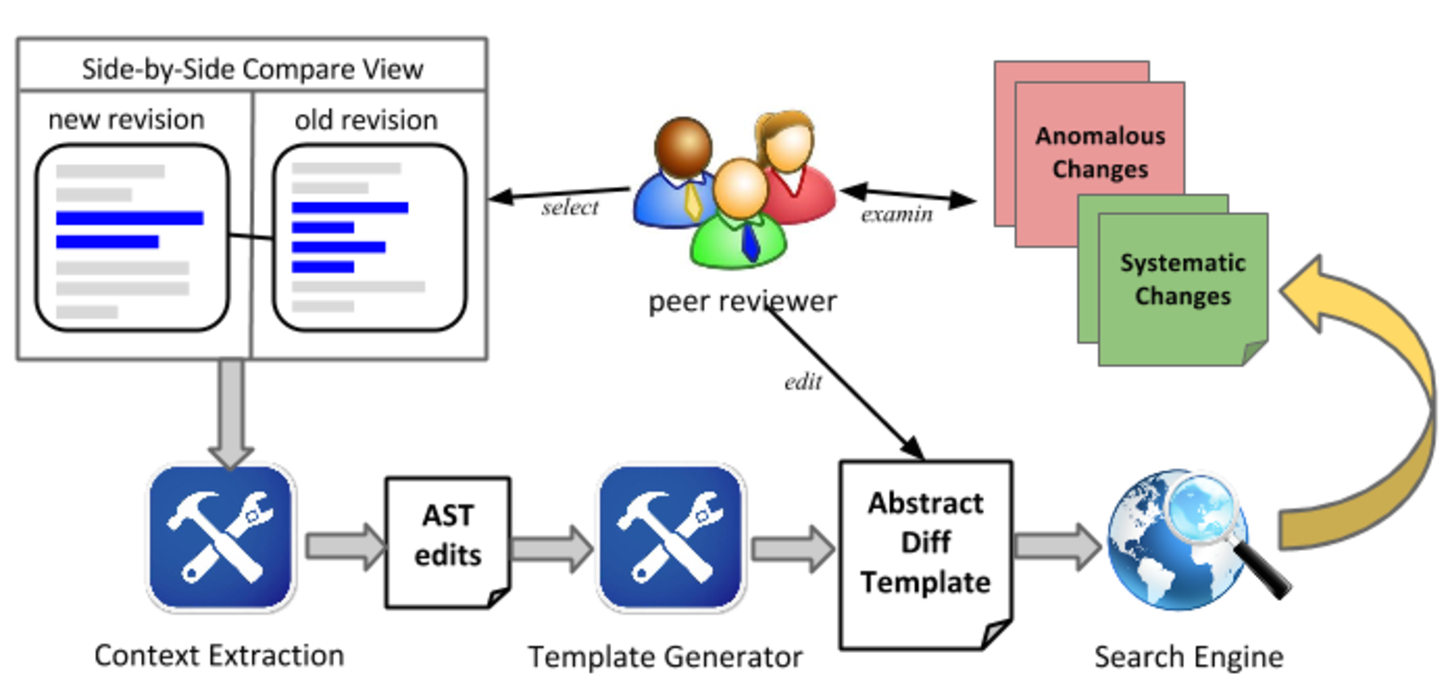
\includegraphics[width=0.8\textwidth]{images/critics-workflow.pdf}
 \caption{The workflow of {\critics}}
 \label{fig:critics-workflow}
\end{figure}

To address this issue, Zhang et al.~present {\critics}, a novel approach that allows reviewers to interactively inspect such systematic changes during peer code review~\cite{zhang2015interactive}. Figure~\ref{fig:critics-workflow} describes the interactive workflow of {\critics}. Given a specified change that a reviewer would like to inspect, {\critics} creates a change template from the selected change, which serves as the pattern for searching similar changes. {\critics} includes {\em change context} in the template---unchanged, surrounding program statements that are relevant to the selected change. {\critics} models the template as Abstract Syntax Tree (AST) edits and allows reviewers to iteratively customize the template by parameterizing its content and by excluding certain statements. {\critics} then matches the customized template against the rest of the codebase to summarize similar changes and locate potential inconsistent or missing changes. Reviewers can incrementally refine the template and progressively search for similar changes until they are satisfied with the inspection results. This interactive feature allows reviewers with little knowledge of a codebase to flexibly explore the program changes with a desired pattern.



\begin{figure}[ht]
 \centering
 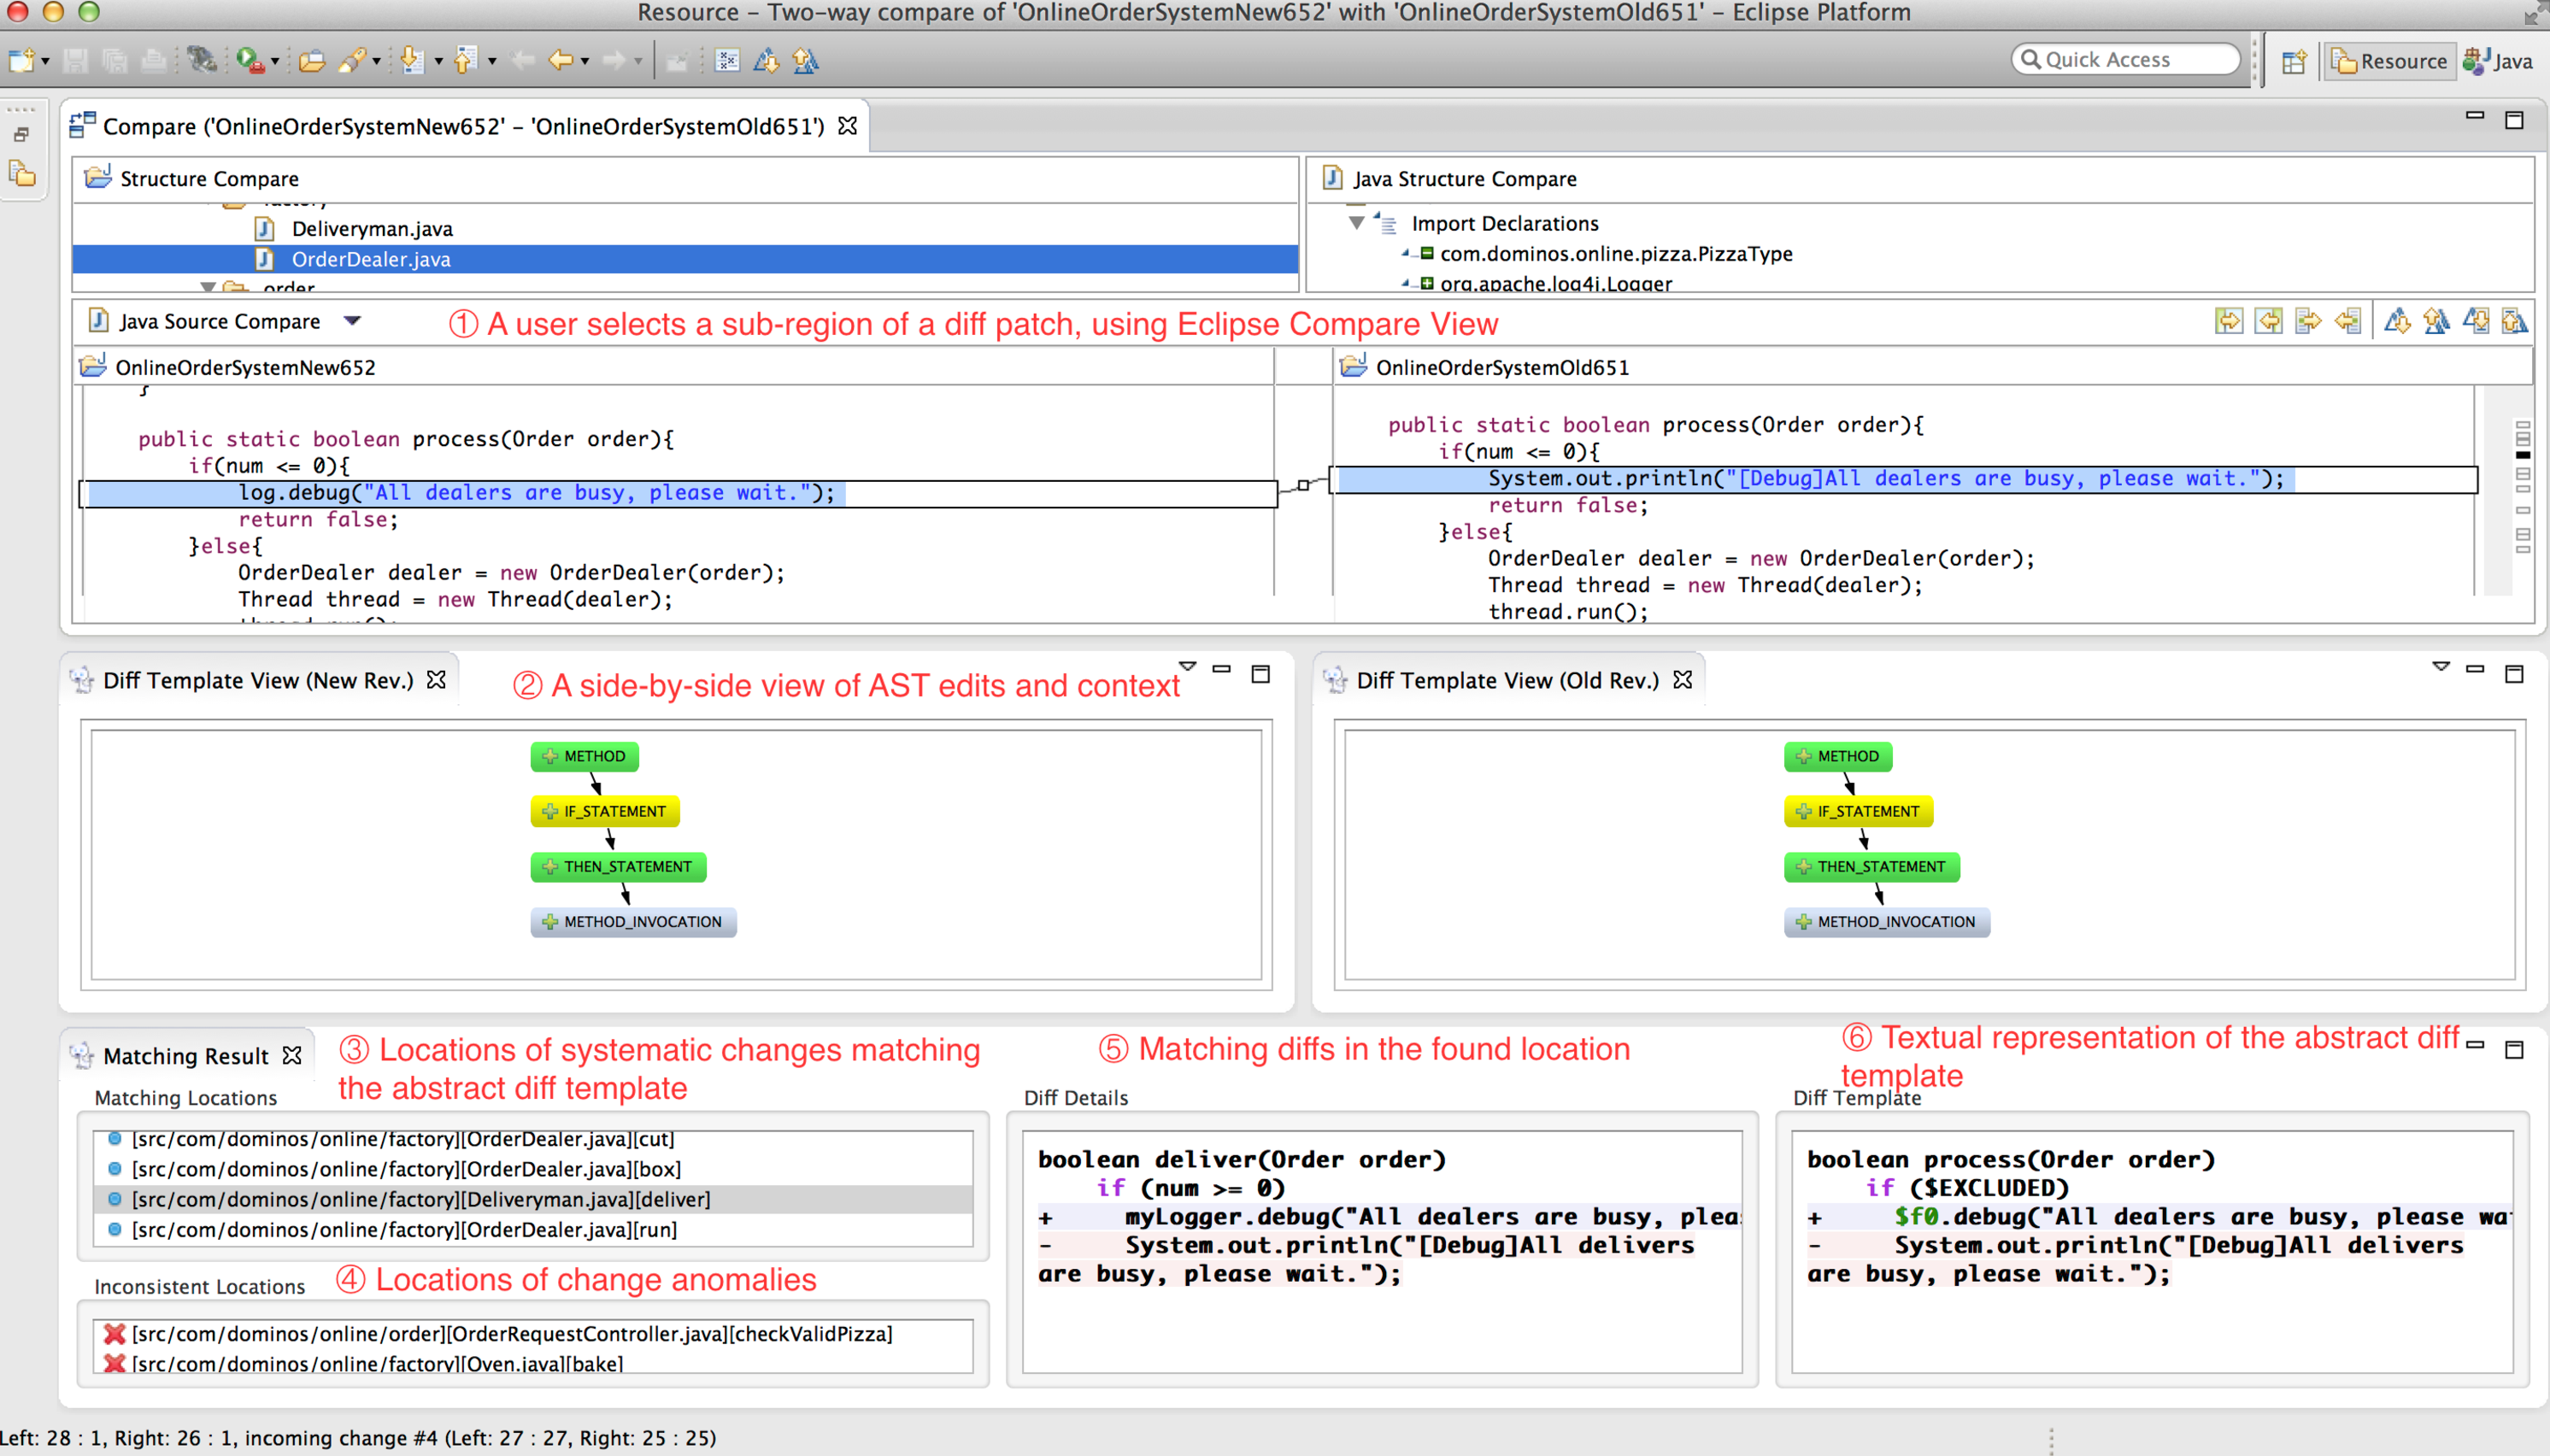
\includegraphics[width=\textwidth]{images/critics-UI.pdf}
 \caption{A screen snapshot of {\critics}'s Eclipse plugin and its features}
 \label{fig:critics-UI}
\end{figure}

{\critics} is implemented as an Eclipse plugin.\footnote{{\critics}'s tool and evaluation dataset are available online \url{https://sites.google.com/a/utexas.edu/critics/}} Figure~\ref{fig:critics-UI} shows a screenshot of {\critics} plugin. {\critics} is integrated with the {\bf Compare View} in Eclipse, which displays line-level differences per file (see \ding{172} in Figure~\ref{fig:critics-UI}). A user can specify a program change she wants to inspect by selecting the corresponding code region in the Eclipse Compare View. The {\bf Diff Template View} (see \ding{173} in Figure~\ref{fig:critics-UI}) visualizes the change template of the selected change in a side-by-side view. Reviewers can parameterize concrete identifiers and exclude certain program statements by clicking on the corresponding node in the Diff Template View. {\bf Textual Diff Template View} (see \ding{177} in Figure~\ref{fig:critics-UI}) shows the change template in a unified format. The {\bf Matching Result View} summarizes the consistent changes as {\em similar changes} (see \ding{174} in Figure~\ref{fig:critics-UI}) and inconsistent ones as {\em anomalies} (see \ding{175} in Figure~\ref{fig:critics-UI}).


\subsubsection{Change Decomposition}

To address this issue, Barnett et al.~present {\clusterchanges}, a lightweight static analysis technique for decomposing large changes. The insight is that program changes that address the same issue can be related via implicit dependency information such as {\em def-use} relationship. For example, if a method definition is changed in one location and its callsites are changed in two other locations, these three changes are likely to be related and should be reviewed together. Given a code review task, {\clusterchanges} first collects the set of definitions for types, fields, methods, and local variables in the corresponding project under review. Then {\clusterchanges} scans the project for all uses (i.e., references to a definition) of the defined code elements. For instance, any occurrence of a type, field, or method either inside a method or a field initialization is considered to be a use. Based on the extracted def-use information, {\clusterchanges} identifies three relationships between program changes. 

 {\bf Def-use relation}. If the definition of a method or a class field is changed, all the uses should also be updated. The change in the definition and the corresponding changes in its references are considered related.
 {\bf Use-use relation}. If two or more uses of a method or a class field defined within the change-set are changed, these changes are considered related. 
 {\bf Enclosing relation}. Program changes in the same method are considered related because a) based on observation, program changes to the same method are often related, (b) reviewers often inspect methods atomically rather than reviewing different changed regions in the same method separately.

Given these relations, {\clusterchanges} creates a partition over the set of program changes by computing a transitive closure of related changes. On the other hand, if a change is not related to any other changes, it will be put into a specific partition, {\em miscellaneous changes}.

\todo{Expand the following technique a little bit more. Give similar weights to ClusterChange.}
Independently from {\clusterchanges}, Tao et al.~present a similar change decomposition technique that leverages more sophisticated heuristics, other than the def-use analysis only~\cite{tao2015partitioning}. Tao et al.~cluster changes based on the following heuristics.

\subsubsection{Refactoring Aware Code Review} 

\paragraph{Refactoring Reconstruction.}  
Demeyer {et al.} first proposed the idea of inferring refactorings from two program versions by comparing two program versions. They used a set of ten characteristic metrics, such as LOC and the number of method calls within a method~\cite{Demeyer2000}. Zou and Godfrey first coined the term origin analysis, which serves as a basis for refactoring reconstruction by matching code elements using multiple criteria (e.g., names, signatures, metric values, callers, and callees)~\cite{Zou2005}. Their approach infers merge, split, and rename refactorings. Van Rysselberghe and Demeyer used a clone detector to detect moved methods~\cite{Rysselberghe2003}.  Antoniol {et al.} identified class-level refactorings using a vector space information retrieval approach~\cite{Antoniol2004}. Malpohl {et al.} \cite{Malpohl2000} align tokens using {\it diff} and infers a function or variable renaming when distinct tokens are surrounded by mapped token pairs. Van Rysselberghe and Demeyer \cite{Rysselberghe01} use a clone detector to detect moved methods. 
 Dig et al.'s approach, {Refactoring Crawler} identifies refactorings in two stages~\cite{Dig2006}. First, it finds a list of code element pairs using {\em shingles} (a metric-based fingerprint) and performs a semantic analysis based on reference relationships (calls, instantiations, uses of types, import statements). The second part of the algorithm is an iterative, fix point algorithm that considers refactorings in a top-down order. 

Wei{\ss}gerber and Diehl's approach~\cite{Weissgerber2006} extracts added and deleted entities (fields, methods, and classes) by parsing deltas from a version control system and then compares these entities based on their {name similarity}. When it cannot disambiguate all refactoring candidates, it uses a {clone detector} (CCFinder~\cite{Kamiya2002}) to rank these candidates. S. Kim et al.'s approach~\cite{SKim2005} considers various information (such as {calling relationships}, {clone detection} results, and {name similarity}) to match method-headers.  Wu et al.'s approach~\cite{Wu2010:aura} is a hybrid approach that combines the strengths of {call-graph matching} and {name-similarity} based matching. Nguyen et al.'s approach~\cite{Nguyen2010:libsync} identifies refactorings in libraries to support adaptation of the client applications that use those libraries. Similar to Xing et al.'s approach, the algorithm matches code elements top-down based on method name similarity and method body contents. Fluri et al.'s approach~\cite{Fluri2007} compares two versions of abstract syntax trees, computes tree-edit operations, and maps each tree-edit to atomic AST-level change types (e.g., parameter ordering change).

Xing et al.'s approach~\cite{Xing2005} UMLDiff extracts class models from two versions of a program, traverses the two models, and identifies corresponding entities based on their {name similarity} and {structure similarity} {(i.e., similarity in type declaration and uses, field accesses, and method calls)}.
Xing {et al.} later presented an extended approach to refactoring reconstruction based on change-facts {\em queries} \cite{Eleni01}. They first extract facts regarding design-level entities and relations from each individual source code version. These facts are then pairwise compared to determine how the basic entities and relations have changed from one version to the next. Finally, queries corresponding to well-known refactoring types are applied to the change-facts database to find concrete refactoring instances.

Prete et al.'s {\em RefFinder} uses a rule-based program differencing approach~\cite{Prete2010:reffinder,Kim2010:reffinder} to reconstruct refactoring from program versions. It encodes 63 out of 72 refactoring types in Fowler's catalog as template logic rules, and uses a logic-query approach to infer concrete refactoring instances~\cite{Prete2010:reffinder}. Prete et al.~use pre-defined logic rules to detect structural differences that fit known refactoring types. It actively leverages the structural constraints of a program before and after each refactoring type and has two advantages. First, RefFinder analyzes the body of methods including changes to the control structure within method bodies. Thus, it can handle the detection of refactorings such as {\it replacing conditional code with polymorphism}. Second, it handles composite refactorings, since the approach reasons about which constituent refactorings must be detected first and reason about how those constituent refactorigs are knit together to detect higher-level, composite refactorings.

\label{sec:intro} 
\begin{figure*}
\centering
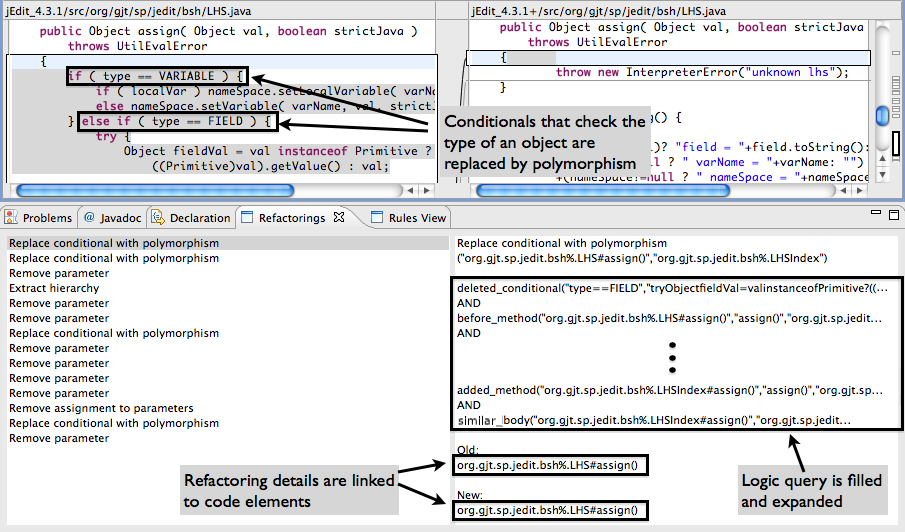
\includegraphics[width=0.95\textwidth]{images/reffinder.png}
\caption{RefFinder infers a {\it replace conditionals with polymorphism} refactoring from change facts {\it deleted\_conditional}, {\it after\_subtype}, {\it before\_method}, {\it added\_method} and {\it similar\_body}.\cite{Kim2010:reffinder}}
 \label{fig:reffinderscreenshot}
\end{figure*}

A developer may begin her investigation by selecting two program versions either from her current workspace projects or revisions from a Subversion repository. RefFinder compares the syntax tree of each version to compute structural change-facts such as \factfont{deleted\-\_trycatch}. RefFinder then invokes template logic queries, each of which encode the structural constraints of a program before and after refactorings. 

Consider a {\it replace conditionals with polymorphism} refactoring example from version 4.3.1 of jEdit, an open source text editor. In the old version, the class \codefont{LHS} contained a method, \codefont{assign()}, whose behavior depended on the value of the \codefont{type} field. The new version of this methods supplants this conditional logic by adding \codefont{LHS}'s subclasses and then using polymorphism to invoke a different behavior by overriding \codefont{assign()} in each of the subclasses.
In order to find a \factfont{replace\_\-conditionals\-\_with\-\_polymorphism(oldmethod, subclass)} refactoring, RefFinder invokes a query \factfont{(deleted\-\_conditional\-(?condition, ?thenpart, ?elsepart, ?superclass) $\wedge$ before\-\_method\-(?oldmethod, ?superclass), after\-\_subtype\-(?superclass, ?subclass) $\wedge$ added\-\_method\-(?newmethod, ?subclass) $\wedge$ similar\-\_body\-(?new\-method, ?oldmethod))}, to check that a type check was performed in the conditional and that the new method body is similar to the original method. In our logic query description, \factfont{?x} indicates an existentially quantified logic variable, \factfont{x}. 
As shown in Figure \ref{fig:reffinderscreenshot}, RefFinder visualizes the reconstructed refactorings as a list.  The panel on the right summarizes key details of the selected refactoring and allows the developer quickly navigate to the associated code fragments. 


%Ref-Finder: a Refactoring Reconstruction Tool based on Logic Query Templates, Miryung Kim, Matthew Gee, Alex Loh, and Napol Rachatasumrit, FSE' 10: Proceedings of the 18th ACM SIGSOFT Symposium on the Foundations of Software Engineering, Pages 371-372, Publisher: ACM DOI, Formal Research Demonstration (local pdf)  

% Refactoring Inspection Support for Manual Refactoring Edits, Everton L.G. Alves, Myoungkyu Song, Tiao Massoni, Patricia D. L. Machado, Miryung Kim, TSE: IEEE Transactions on Software Engineering, 20 pages (Accepted, March 2017) (link) 

\paragraph{Refactoring Validation.} Schaeffer et al.~validate refactoring edits by comparing data and control dependences between two program versions~\cite{Schaefer2010:refactoring}. As opposed to validating refactoring edits, Daniel et al. focus on testing refactoring engines by systematically generating input programs for refactoring transformations~\cite{Brett2007:reftest}. 

Regression testing is the most used strategy for checking refactoring correctness. However, Rachatasumrit and Kim~\cite{rachatasumrit2012empirical} find that test suites are often inadequate and developers may hesitate to initiate or perform refactoring tasks due to inadequate test coverage~\cite{kim2012field}. Soares et al.~\cite{Soares:icse2010} design and implement SafeRefactor that uses randomly generated test suites for detecting refactoring anomalies. Mongiovi et al.~\cite{mongiovi2013making} introduces SafeRefactorImpact. SafeRefactorImpact extends SafeRefactor by adding an impact analysis step. SafeRefactorImpact decomposes an edit into small-grained transformations and analyzes the impact of each one. Then, it uses Randoop to generate test cases for the impacted methods. In our studies, we show that even tool-generated tests can be inadequate. Using a SafeRefactor like testing validation, we find that about 25\% of the refactoring anomalies are not identified by using generated test suites, even with a long generation time limit (100 seconds). 

Formal verification is an alternative for avoiding refactoring anomalies~\cite{mens2004survey}. Corn\'elio et al.~\cite{cornelio2010sound} propose rules for guaranteeing semantic preservation. Similarly, Mens et al.~\cite{mens2005formalizing} use graph rewriting for specifying refactorings. Overbey et al.~\cite{overbey2010collection} present a collection of refactoring specifications for Fortran 95. However, these approaches focus on improving the correctness of automated refactoring through formal specifications, as opposed to finding anomalies during manual refactoring. 


RefDistiller is a static analysis approach~\cite{Alves2017:refdistiller,Alves:2014:RRA:2635868.2661674} to support the inspection of manual refactorings. It combines two techniques. First, it applies predefined templates to identify potential missed edits during manual refactoring. Second, it leverages an automated refactoring engine to identify extra edits that might be incorrect, helping to  determine the root cause of detected refactoring anomalies.

GhostFactor~\cite{geManual2014} checks the correctness of manual refactoring, similar to RefDistiller. 
However, unlike RefDistiller, GhostFactor does not have any capability to isolate potential behavior changes from pure refactoring by running an equivalent automated refactoring. GhostFactor detects missing edits only, while RefDistiller detects both missing and extra edits. 

Ge and Murphy-Hill~\cite{ge2014towards} propose a refactoring-aware code review tool, with goals similar to RefDistiller. This tool helps reviewers by identifying applied refactorings and letting developers examine them in isolation. Ge and Murphy-Hill leverage Eclipse refactoring APIs to separate pure refactorings. RefDistiller goes a step further by extending Eclipse refactoring APIs to prevent unsafe refactoring by checking bug conditions, allowing to apply automated refactoring in a safe manner when isolating pure refactoring. 


Other approaches ensure the consistency between refactored programs and other software artifacts like design models~\cite{Bottoni2003:coordinatedTransformation,Straeten2003:UML}. For example, Bottoni et al.~modeled a refactoring as a set of distributed graph transformations~\cite{Bottoni2003:coordinatedTransformation}. Each time a code refactoring is applied, the corresponding graph transformations are automatically applied to related design models to preserve consistency. Van Der Straeten et al.~suggested using description logic to maintain the consistency between relevant UML models as they evolve~\cite{Straeten2003:UML}.


\paragraph{\bf Detecting Inconsistent Changes to Clones} 
\todo{ASE 2013 paper} 


\paragraph{\bf Change Conflicts, Interference, and Relevance. } 
Most version control systems are only able to detect most simple types of conflicting changes\textemdash changes made on top of other changes~\cite{Mens2002}. Men's survey on software merging lists various conflict and interference detection models and algorithms~\cite{Mens2002}. To detect changes that indirectly conflict with each other, Horwitz et al. developed a semantics based tool that automatically integrates non-interfering versions by using program slicing on program dependence graphs to determine if there is interference. They provide, however, no empirical evidence on how often non-interference occurs. As another example, Shao et al.'s research on semantic interference detection checks the overlap between the data-dependence based impact sets of parallel updates~\cite{Shao2007:interference}.  Furthermore, various approaches have defined change impacts at a different granularity and implemented static and dynamic analyses for computing the impact of a code change~\cite{Apiwattanapong2005, Arnold1996:impact, Elbaum2001, Orso2003, Orso2004:impact, Ren2004}.  

Existing techniques that can identify related changes across revisions rely on temporal proximity \cite{Bevan2005, Fischer2003, German2004:softchange, Zimmermann2004b}, syntactic dependence \cite{Chesley2005}, physical location \cite{Zeller1999}, committer information \cite{Fischer2003, German2004:softchange, Zimmermann2004b}, history of co-changes \cite{Gall1998, Ying2004, Zimmermann2004}, and content similarity~\cite{Kim2009, Nguyen2009:clever} and other heuristics \cite{Zeller1999}. For example, Crisp \cite{Chesley2005} computes atomic structural changes such as method additions and deletions via AST differencing and groups syntactically dependent changes through def-use relationships. As various notions of delta-relationships (e.g., interference, dependence, and similarity, co-occurrence) can be used to identify relevant software modifications,  
\paragraph{Comprehending Structural Dependencies} 
Representing a program's code elements and structural dependencies as a set of logic facts has been used for decades. Grok \cite{Holt1998} extracts facts about code elements and structural relationships in software and supports querying the resulting relational databases. CodeQuest \cite{Hajiyev2006} automatically evaluates logic queries specified by programmers to assist program investigation. Mens et al.'s intentional view \cite{Mens2002b} allows programmers to specify concerns or design patterns using logic rules. Eichberg et al. \cite{Eichberg2008} use Datalog rules to continuously enforce constraints on structural dependencies as software evolves. DeMIMA~\cite{Gueheneuc2008:demima} finds concrete instantiations of design patterns by matching the skeleton of design patterns against a program structure. Tourw{\'e} {et al.} \cite{Tourwe01} use logic meta-programming to detect bad smells to identify which parts of a system needs to be refactored.

\paragraph{Maintaining Awareness about Software Changes} 
As development teams become distributed, and the size of the system is often too large to be handled by a few developers, multiple developers often work on the same module at the same time. In addition, the market-pressure to develop new features or products makes parallel development no longer an option.
Professor Perry's study on a subsystem of Lucent 5ESS telephone found that 12.5\% of all changes are made by different developers to the same files within 24 hours, showing a high degree of parallel updates~\cite{Perry2001:parallel}. A subsequent study by Shao et al. found that even though only 3\% of the changes made within 24 hours by different developers physically overlapped each other's changes at a textual level but there was a high degree of semantic interference among parallel changes at a data flow analysis level (about 43\% of revisions made within one week). They also discovered a significant correlation between files with a high degree of parallel development and the number of defects~\cite{Shao2007:interference}. 

% Informaition Needs: Ko et al.~\cite{Ko2007} studied software engineers' information needs by observing their daily activities and analyzing observation logs. Sillito and Murphy~\cite{Sillito2008} studied the types of questions that programmers ask to assess how well existing tools support those questions. Software engineers often need to be aware of other programmers' activities so as to avoid overlapping effort,  prevent potential conflicts, identify experts, discover opportunities for ad-hoc collaboration, and find a common ground for further communication \cite{Dourish1992, Herbsleb2007:global, Sarma2008}. 

Workspace awareness systems such as FASTDash \cite{Biehl2007} and CollabVS~\cite{Hegde2008:collabVS} provide information about other developers' task status or activities. Palantir \cite{Sarma2003} and Lighthouse \cite{daSilva2006} can assist programmers in detecting structural conflicts early by monitoring changes in other programmers' workspace in real-time. Nightwatch \cite{OReilly2003} and CVS-Watch \cite{Berliner1990:cvs2} monitor other developers' activities using programmer-specified watch-points. These existing approaches either overload programmers with a large number of change-events or require substantial effort by programmers to specify what they want to monitor. YooHoo~\cite{Holmes2010:Yoohoo} mitigates this problem in some degree by filtering out changes according to predefined rules; however, it limited to API declaration changes that lead to build errors. 

 
\noindent {\bf Search and Visualization of Software Changes. }
SCM query systems such as SCQL \cite{Hindle2005} or CVS Query \cite{bonsai} can search check-ins based on who changed which file and when, but cannot search change history by code elements and dependencies. Systems such as Hipikat \cite{Cubranic2003}, Bridge \cite{Venolia2006:bridge}, Tesseract \cite{Sarma2009:tesseract}, and Deep Intellisense \cite{Holmes2008:intellisense} automatically associate different types of software artifacts (e.g., check-ins, bug reports, and emails) but provide limited help in querying code changes. 


Several visualization tools focus on representing changes between versions \cite{Ball1996,Eick2002,Girba2004,Holt1996,Lanza2001,Lanza2003,Rysselberghe2004a}. For example, Evolution Matrix \cite{Lanza2001} visualizes classes that have been added, modified, and deleted in different versions and creates a 2-D matrix where the rows represent classes and the columns represent the versions of the artifact. These tools generally require substantial interpretation effort by developers to understand system evolution. Studying program evolution by analyzing existing software project artifacts is increasingly becoming a popular research approach. Existing research infrastructures for mining software artifacts focus on data extraction \cite{Bevan2005,Fischer2003} and integration of different types of software artifacts \cite{Cubranic2003, Venolia2006:bridge, Sarma2009:tesseract, Begel2010:codebook}. 

\subsection{Program Differencing} 
Existing program differencing techniques use similarities in names and structure to match code elements at a particular granularity: (1) lines and tokens \cite{Apostolico1997, Hunt1977, Reiss2008, Tichy1984}, (2) abstract syntax tree nodes \cite{Cottrell2007, Fluri2007, Hunt2002, Neamtiu2005, Raghavan2004, Yang1991}, (3) control flow graph nodes \cite{Apiwattanapong2004, Laski1992}, (4) program dependence graph nodes \cite{Binkley1995, Horwitz1990, Jackson1994}, etc.  For example, the ubiquitous tool {\it diff} computes line-level differences per file using the longest common subsequence algorithm \cite{Hunt1977}. These tools output individual additions and deletions at a particular granularity without any structure, obliging the developer to read individual differences. Some approaches attempt to mitigate this problem by grouping the differences by physical locations (directories and files) \cite{Hunt1976}, by logical locations (packages, classes, and methods) \cite{Xing2005}, by structural dependencies (define-use and overriding) \cite{Chesley2005}, or by similarity of names. 
As existing approaches do not recognize regularities in code changes, subsequently they are unable to detect inconsistencies in code changes, leaving it to a programmer to discover potential bugs.  

\subsection{Code Matching} 
		\label{related_codematching}
\indent{\textit{Suppose that a program $P'$ is created by modifying $P$. Determine the difference $\Delta$ between $P$ and $P'$. For a code fragment $c' \in P'$, determine whether $c' \in \Delta$. If not, find $c'$'s corresponding origin $c$ in $P.$}}

A code fragment in the new version either contributes to the difference or comes from the old version. If the code fragment has a corresponding origin in the old version, it means that it does not contribute to the difference. Thus, finding the delta between two versions is the same problem as finding corresponding code fragments between two versions. 
Suppose that a programmer inserts if-else statements in the beginning of the method \codefont{m\_A} and reorders several statements in the method \codefont{m\_B} without changing semantics (see Table \ref{code}). An intuitively correct matching technique should produce [(s1-s1'), (s2-s2'), (s3-s4'), (s4-s3'), and (s5-s5')] and identify that s0' is added.  
\begin{table} 
\footnotesize
\caption{Example code change}
\begin{tabular}{|p{0.50\textwidth}|p{0.50\textwidth}|} \hline
before & after \\ \hline
\begin{verbatim} 
mA (){
  if (pred_a) { //s1
    foo(); //s2
  } 
}
mB (b){ 
  a= 1; //s3
  b= b+1; //s4
  fun(a,b); //s5
} \end{verbatim} 
& 
\begin{verbatim} 
mA (){
  if (pred_a0) { //s0'
    if (pred_a) { //s1'
      foo(); //s2'
    } 
  }
}
mB (b){ 
  b= b+1; \\s3'
  a= 1; \\s4'
  fun(a,b); \\s5'
}\end{verbatim} \\ \hline
\end{tabular} 
\label{code} 
\end{table}


Matching code across program versions poses several challenges. 
First, previous studies \cite{SKim2005} indicate that programmers often disagree about the origin of code elements; low inter-rater agreement suggests that there may be no ground truth in code matching.
Second, renaming, merging, and splitting of code elements make the matching problem non-trivial. Suppose that a file \codefont{PElmtMatch} changed its name to \codefont{PMatching}; a procedure \codefont{matchBlck} is split into two procedures \codefont{matchDBlck} and \codefont{matchCBlck}; and a procedure \codefont{matchAST} changed its name to \codefont{matchAbstractSyntaxTree}. 
The intuitively correct matching technique should produce [(\codefont{PElmtMatch, PMatching}), (\codefont{matchBlck, matchDBlck}), (\codefont{matchBlck, matchCBlck}), \\and (\codefont{matchAST, matchAbstractSyntaxTree})], 
while simple name-based matching will consider \codefont{PMatching}, \codefont{matchDBlck}, \codefont{matchCBlck}, and \codefont{matchAbstractSyntaxTree} added and consider \codefont{PElmtMatch}, \codefont{matchBlck}, and \codefont{matchAST} deleted.

Existing code matching techniques usually employ syntactic and textual similarity measures to match code. They can be characterized by the choices of (1) an underlying program representation, (2) matching granularity, (3) matching multiplicity, and (4) matching heuristics. This section explains how the choices impact applicability, effectiveness, and accuracy of each matching method by creating an evaluation framework. 


\paragraph{Entity Name Matching}
The simplest matching method treats code elements as immutable entities with a fixed name and matches the elements by name. For example, Zimmermann et al. model a function as a tuple, \textit{(file name, FUNCTION, function name)}, and a field as a tuple, \textit{(function name, FIELD, field name)} \cite{Zimmermann2004}. Similarly, Ying et al. \cite{Ying2004} model a file with its full path name. %In fact, matching by name would be sufficient for many evolution analyses that intend to identify coarse-grained patterns such as the characteristics of fault prone modules \cite{Eick2001,Graves2000,Nagappan2005}.  

\paragraph{String Matching}
When a program is represented as a string, the best match between two strings is computed by finding the longest common subsequence (LCS) \cite{Apostolico1997}. The LCS problem is built on the assumption that (1) available operations are addition and deletion, and (2) matched pairs cannot cross one another. Thus, the longest common subsequence does not necessarily include all possible matches when available edit operations include copy, paste, and move. Tichy's \textit{bdiff} \cite{Tichy1984} extended the LCS problem by relaxing the two assumptions above: permitting crossing block moves and not requiring one-to-one correspondence. 

The line-level LCS implementation, \textit{diff} \cite{Hunt1977} is fast, reliable, and readily available. Thus, it has served as a basis for popular version control systems such as CVS.\footnote{http://www.cvshome.org} or Subversion\footnote{http://subversion.tigris.org} Many evolution analyses are based on {\it diff} because they use version control system data as input. Identification of fix-inducing code snippets \cite{Sliwerski2005} is also based on tracking \textit{(file name:: function name:: line number)} backward from the moment that a bug is fixed.  

% S. Reiss  (Tracking Source Locations in ICSE 2008 
Reiss \cite{Reiss2008} evaluated practical LCS-based source line tracking techniques. His investigation shows that the {\it W\_BEST\_LINE} method\textemdash  a variation of LCS algorithm that considers $k$ number of contextual lines\textemdash is about as effective as any other method but is faster and requires only a small amount of storage. This method compares each line to derive a normalized match value between zero (no match) and one (exact match); looks at a context consisting of $k/2$ lines before and after the line; and counts the number of these lines that match the corresponding line in the new version.  

% Canfora et al. 
Recently, Canfora et al. \cite{Canfora2007} developed a source line technique that takes differencing results from {\it diff}-based version control systems as input and identifies changed-lines in addition to added- and deleted-lines. This technique first computes hunk similarity between every possible hunk pair using a vector space model and then computes the Levenstein distance \cite{Levenstein1966} to map source lines within the mapped hunk pairs. In contrast to {\it diff}, this approach detects changed-lines in addition to deleted- and added-lines. 



\paragraph{Syntax Tree Matching}
For software version merging, Yang \cite{Yang1991} developed an AST differencing algorithm. Given a pair of functions $(f_T,f_R)$, the algorithm creates two abstract syntax trees $T$ and $R$ and attempts to match the two tree roots. Once the two roots match, the algorithm aligns $T$'s subtrees ${t_1, t_2, ..., t_i}$ and $R$'s subtrees ${r_1, r_2, ... r_j}$ using the LCS algorithm and maps subtrees recursively. This type of tree matching respects the parent-child relationship as well as the order between sibling nodes, but is very sensitive to changes in nested blocks and control structures because tree roots must be matched for every level. 

For dynamic software updating, Neamtiu et al. \cite{Neamtiu2005} built an AST-based algorithm that tracks simple changes to variables, types, and functions. Neamtiu's algorithm assumes that function names are relatively stable over time. 
It
traverses two ASTs in parallel;
matches the ASTs of functions with the same name; 
and incrementally adds one-to-one mappings as long as the ASTs have the same shape. In contrast to Yang's algorithm, it cannot compare structurally different ASTs. 

% Change Distiller 
Fluri et al.'s Change Distiller \cite{Fluri2007} uses an improved version of Chawathe et al.'s hierarchically structured data comparison algorithm \cite{Chawathe1996}. Change Distiller takes two abstract syntax trees as input and computes basic tree edit operations such as {\it insert, delete, move} or {\it update} of tree nodes. It uses {\it bi-gram string similarity} to match source code statements such as method invocations and uses {\it subtree similarity} to match source code structures such as if-statements. After identifying tree edit operations, Change Distiller maps each tree-edit to an atomic AST-level change type. 

% R. Walker 
Cottrell et al.'s Breakaway \cite{Cottrell2007} automatically identifies detailed structural correspondences between two abstract syntax trees to help programmers generalize two pieces of similar code. Its two-pass greedy algorithm is applied to ordered child list properties (statements in a block) then to unordered nodes (method declarations). 

Finally, the following two techniques do not directly compare ASTs but use syntactic information to guide string level differencing. 
% Hunt Tichy 
Hunt and Tichy's 3-way merging tool \cite{Hunt2002} parses a program into a language neutral form; compares token strings using the LCS algorithm; and finds syntactic changes using structural information from the parse.
% Raghavan 
Raghavan et al.'s Dex \cite{Raghavan2004} locates the changed parts in C source code files using {\it patch} file information and feeds the changed parts into a tree differencing algorithm to output the edit operations. 


\paragraph{Control Flow Graph Matching}
Laski and Szermer \cite{Laski1992} first developed an algorithm that computes one-to-one correspondences between CFG nodes in two programs. This algorithm reduces a CFG to a series of single-entry, single-exit subgraphs called hammocks and matches a sequence of hammock nodes using a depth first search (DFS). Once a pair of corresponding hammock nodes is found, the hammock nodes are recursively expanded in order to find correspondences within the matched hammocks. 
 
\textit{Jdiff} \cite{Apiwattanapong2004} extends Laski and Szermer's (LS) algorithm to compare Java programs based on an enhanced control flow graph (ECFG). 
\textit{Jdiff} is similar to the LS algorithm in the sense that hammocks are recursively expanded and compared, but is different in three ways: 
First, while the LS algorithm compares hammock nodes by the name of a start node in the hammock, \textit{Jdiff} checks whether the ratio of unchanged-matched pairs in the hammock is greater than a chosen threshold in order to allow for flexible matches.
Second, while the LS algorithm uses DFS to match hammock nodes, \textit{Jdiff} only uses DFS up to a certain look-ahead depth to improve its performance. 
Third, while the LS algorithm requires hammock node matches at the same nested level, \textit{Jdiff} can match hammock nodes at a different nested level; thus, \textit{Jdiff} is more robust to addition of while loops or if-statements at the beginning of a code segment. \textit{Jdiff} has been used for regression test selection \cite{Orso2004} and dynamic change impact analysis \cite{Apiwattanapong2005}. 

CFG-like representations are commonly used in regression test selection research. Rothermel and Harrold's algorithm \cite{Rothermel1997} traverses two CFGs in parallel and identifies a node with unmatched edges, which indicates changes in code. In other words, the algorithm stops parallel traversal as soon as it detects changes in a graph structure; thus, this algorithm does not produce deep structural matches between CFGs. However, traversing graphs in parallel is still sufficient for the regression testing problem because it conservatively identifies affected test cases. In practice, regression test selection algorithms \cite{Harrold2001, Orso2004} require that syntactically changed classes and interfaces are given as input to the CFG matching algorithm. 

\paragraph{Program Dependence Graph Matching}
There are several program differencing algorithms based on a program dependence graph \cite{Horwitz1990, Binkley1995, Jackson1994}. 

Horwitz \cite{Horwitz1990} presents a semantic differencing algorithm that operates on a program representation graph (PRG) which combines features of program dependence graphs and static single assignment forms. In her definition, semantic equivalence between two programs $P1$ and $P2$ means that, for all states $\sigma$ such that $P1$ and $P2$ halt, the sequence of values produced at $c1$ is identical to the sequence of values produced at $c2$ where $c1$ and $c2$ are corresponding locations. 
% Static single assignment form means a control flow augmentation by adding special phi vertices so that each use of a variable in an assignment statement, an ouput statement or a predicate is reach by exactly one definiton.
%Using this notion of semantic equivalence, she developed an algorithm that identifies correspondence between the vertices of $P1$'s PRG and the vertices of $P2$'s PRG. 
Horwitz uses Yang's algorithm \cite{Yang1989} to partition the vertices into a group of semantically equivalent vertices based on three properties, (1) the equivalence of their operators, (2) the equivalence of their inputs, (3) the equivalence of the predicates controlling their evaluation. The partitioning algorithm starts with an initial partition based on the operators used in the vertices. Then by following flow dependence edges, it refines the initial partition if the successors of the same group are not in the same group. Similarly, it further refines the partition by following control dependence edges. If two vertices in the same partition are textually different, they are considered to have only a {\it textual change}. If two vertices are in different partitions, they have a {\it semantic change}. After the partitioning phase, the algorithm finds correspondences between $P1$'s vertices and $P2$'s vertices that minimize the number of semantically or textually changed components of $P2$. 
% semantic change: no matching partition. 
% textual change: same partition but different text. 
% same: same partition and same text. 

Binkley et al. \cite{Binkley1995} presents a 3-way merging algorithm that is based on semantic differences. This algorithm does not find corresponding elements between two versions of a program, but rather makes an assumption that a special editor is used to tag each PDG node to identify added nodes, deleted nodes and changed nodes. Given PDG node level correspondence among three input programs A, B, and Base, the integration algorithm produces a program M that integrates the difference A from Base, the difference B from Base, and the preserved behavior among A, B, and Base. The behavior differences between A and B are approximated by the slice of $AP_{A,Base}$ in $G_A$ where $AP_{A,Base}$ is a set of vertices of $G_A$ whose program slice is different from $G_{Base}$'s slice. Although the problem of determining  whether $G_M$ corresponds to some program is NP-complete, Binkley et al. presented a backtracking algorithm that behaves satisfactorily on actual programs. 

In general, PDG-based algorithms are not applicable to popular modern program languages because they can run only on a limited subset of C-like languages without global variables, pointers, arrays, or procedures. 


\paragraph{Clone Detection} 
A clone detector is simply an implementation of an arbitrary equivalence function. The equivalence function defined by each clone detector depends on a program representation and a comparison algorithm. Most clone detectors are heavily dependent on (1) hash functions to improve performance, (2) parametrization to allow flexible matches, and (3) thresholds to remove spurious matches. A clone detector can be considered as a many-to-many matcher based solely on content similarity heuristics. 

\paragraph{Model Differencing} 
In addition to these, several differencing algorithms compare model elements~\cite{Xing2005, Ohst2003:umldiff, Soto2006:deltaprocess}. For example, UMLdiff~\cite{Xing2005} matches methods and classes between two program versions based on their name. However, these techniques assume that no code elements share the same name in a program and thus use name similarity to produce one-to-one code element matches.  VDiff~\cite{Duley2012:vdiff,Duley2010:vdiff} differs from these by not relying on one-to-one matching based on name similarity. 
\todo{Description of VDiff}

As different language semantics lead to different program differencing requirements, some have developed a general, meta-model based, configurable program differencing framework~\cite{Schmidt2008:sidiff, EMF}. For example, SiDiff \cite{Schmidt2008:sidiff, Treude2007:sidiff} allows tool developers to configure various matching algorithms such as identity-based matching, structure-based matching, and signature-based matching by defining how different types of elements need to be compared and by defining the weights for computing an overall similarity measure.

\subsubsection{Recording Changes} 
Recorded change operations can be used to help programmers reason about software changes. We first describe techniques that capture change operations in an editor or an integrated development environment. Next we describe source code transformation languages, which can serve as a basis for capturing high-level semantic transformations. 


\paragraph{Edit Capture and Replay} 
%purpose
Several editors or integrated development environment (IDE) extensions capture and replay keystrokes, editing operations, and high-level update commands to use the recorded change information for intelligent version merging, studies of programmers' activities, and automatic updates of client applications. 

% example
For example, Dig et al.'s MolhadoRef \cite{Dig2007} automatically resolves merging conflicts that a regular {\it diff}-based merging algorithm cannot resolve by taking into account the semantics of recorded move and rename refactorings. This algorithm extends Lippe's operation-based merging \cite{Lippe1992} by defining a model of merging conflicts in case of rename and move refactorings. While Lippe's operation-based merging only defined abstract change operations and did not have a means of recording change operations in IDE, MolhadoRef implements refactoring-aware version merging by recording refactoring commands in the Eclipse IDE.\footnote{Refactoring-aware version merging is one instance of version merging algorithms. A survey of version merging algorithms and tools is described in \cite{Mens2002}.}

Henkel and Diwan's CatchUp \cite{Henkel2005} captures API refactoring actions as a developer evolves an API and allows the users of the API to replay the refactorings to bring their client software up to date. 

Robbes \cite{Robbes2007} extended a small talk IDE to capture AST-level change operations (creation, addition, removal and property change of an AST node) as well as refactorings. He used the recorded changes to study when and how programmers perform refactorings. Spyware~\cite{Robbes2008:spyware} captures refactorings during development sessions in an IDE rather than trying to infer refactorings from two program versions. Refactoring reconstruction can complement recorded refactorings by providing information about the types of refactorings that are not directly supported by IDEs.


Evans et al. \cite{Evans2003} collected students' programming data by capturing keystroke, mouse and window focus events generated from the Windows operating system and used this data to observe programming practices. Similarly, Kim et al.~\cite{Kim2004} studied copy and paste programming practices by recording keystrokes and edit operations in an Eclipse IDE. 

% granularity -> limitations 
When recorded change operations are used for helping programmers reason about software changes, this approach's limitation depends on the granularity of recorded changes. If an editor records only keystrokes and basic edit operations such as cut and paste, it is a programmer's responsibility to raise the abstraction level by grouping keystrokes. If an IDE records only high-level change commands such as refactorings, programmers cannot retrieve a complete change history. 
In general, capturing change operations to help programmers reason about software change is {\it impractical} as this approach constrains programmers to use a particular IDE. 


\section{An Organized Tour of Seminal Papers: III. Change Validation} 
\label{sec:debugtest}

\begin{figure}[ht]
 \centering
 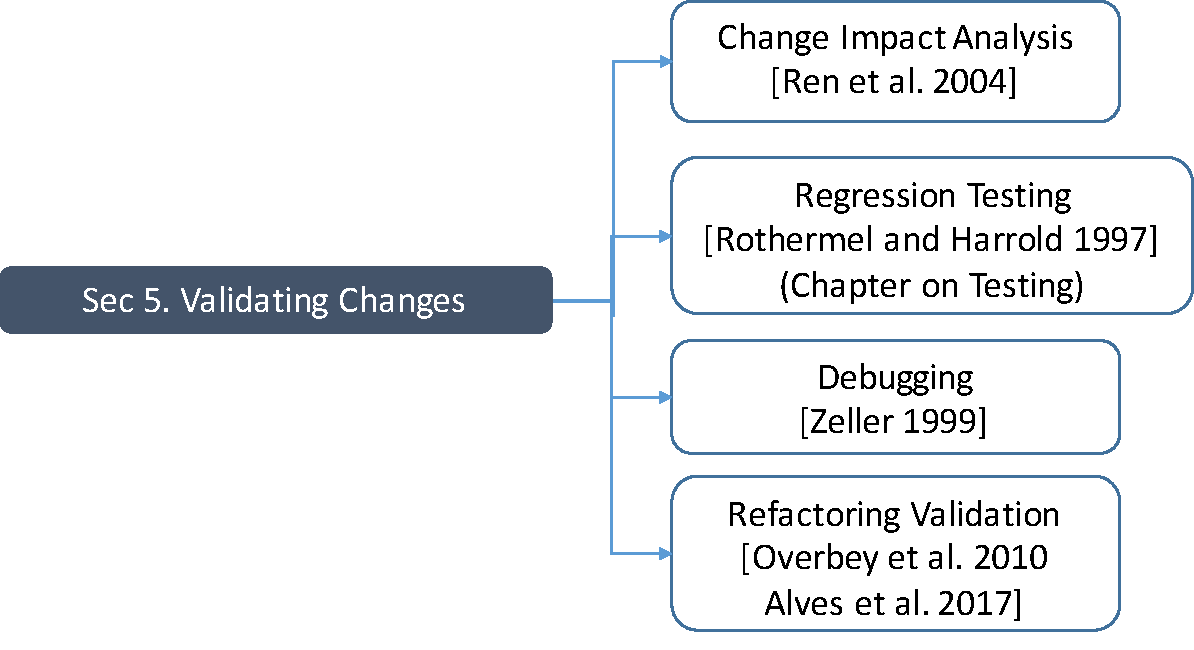
\includegraphics[width=0.6\textwidth]{images/ChangeValidation.pdf} 
 \caption{Change Validation and Related Research Topics} 
 \label{fig:changevalidation} 
\end{figure}

\paragraph{Change Impact Analysis} 

Change Impact Analysis~\cite{bohner1996software, law2003whole, orso2003leveraging, orso2004empirical, ryder2001change, ren2004chianti, ren2006identifying} aims to determine the impact of source code edits on programs under test. Existing techniques, such as Chianti~\cite{ryder2001change,ren2004chianti, ren2006identifying}, select a subset of regression tests whose behavior might have been influenced by program edits and then identify affecting program edits that might related to test failures.  More specifically, Chianti~\cite{Ren2004} constructs dynamic call graphs, modeling programs at a coarser granularity. It compares the syntax tree of the old and new program versions and decomposes the edits into atomic changes at a method and field level~\cite{Ren2004} such as \textsf{AM} for an method addition and \textsf{CM} for method body edits. It reports {\bf affected tests}\textemdash a subset of regression tests relevant to edits and {\bf affecting changes}\textemdash a subset of changes relevant to the execution of affected tests in the new version. 

Chesley et al.~\cite{chesley2005crisp} propose Crisp, which uses four pre-defined rules to group relevant edits based on compilation dependences. However, this technique still requires manual debugging to localize failure-inducing changes. Stoerzer et al.~\cite{stoerzer2006finding} use change classification techniques to find failure-inducing changes. However, this technique does not rank changes, and the classified changes might still be large in number. 

\paragraph{Regression Testing} 
Existing regression test selection algorithms take two program versions $V_1$ and $V_2$, and a test suite $T$ as input and select $tests \in T$ relevant to the delta between $V_1$ and $V_2$. Some algorithms such as DejaVoo~\cite{Rothermel1997, Harrold2001, Orso2004} construct control flow graphs (CFG) for both versions and simultaneously traverse the two graphs to identify matching CFG nodes, $\{(o_1, n_1), (o_2, n_2), \ldots (o_k, n_k)\}$, whose outgoing edges have different targets. Then the tests that exercised any of \{$o_1$, $o_2$, \ldots $o_k$\} are selected as {\em affected tests} because the changes to its control flow may lead to different run-time behavior in the new version $V_2$. 

\paragraph{Delta Debugging.} 
Delta Debugging~\cite{zeller1999yesterday, zeller2001automated} iteratively applies a subset of all changes to
construct intermediate versions to find a minimum set of changes that lead to
a test failure. However, Delta Debugging considers all changes between
the old and new program version as the candidate set without considering compilation dependences among those changes. Furthermore,
Delta Debugging does not rank these edits according to their test spectra, leaving it to a
programmer to sort out a real culprit of a regression test failure among a
large set of potential failure-inducing changes.


\paragraph{Spectra-based Debugging for Changes} 
Spectrum-based fault localization techniques~\cite{hao2005similarity, hao09:interactive, jones2005empirical, abreu2007accuracy, baudry2006improving, liblit2005scalable, yu2008empirical, abreu2009practical} such as Tarantula~\cite{jones2002visualization} statistically compute suspiciousness scores for statements based on execution traces of both passed and failed test cases, and rank potential faulty statements based on the derived suspiciousness scores. Recently, researchers have also introduced more suspiciousness computation measures to the realm of fault localization for localizing faulty statements~\cite{naish2011model, lo2010comprehensive}. For example, Lucia et al.~\cite{lo2010comprehensive} introduced 20 association measures to the area of spectrum-based fault localization and compare them against Tarantula~\cite{jones2002visualization} and Ochiai~\cite{abreu2007accuracy}. Researchers have also developed various automated tool-sets which embodies different spectrum-based fault localization techniques~\cite{tarantula-url, janssen2009zoltar}. However, such spectrum-based fault localization techniques are not scalable to large evolving software systems, as they compute spectra on all statements in each program version and do not leverage information about program edits between the old and new versions.

FaultTracer~\cite{zhang2011localizing}, combines the strengths of Chianti-style change impact analysis and Tarantula-style fault localization. To present a ranked list of potential failure-inducing edits, FaultTracer applies a set of spectrum-based ranking techniques to the affecting changes determined by Chianti-style change impact analysis. It uses a new enhanced call graph representation to measure test spectrum information directly for field-level edits and to improve upon the existing Chianti algorithm. Ren et al.~\cite{ren2007heuristic} propose a heuristic ranking algorithm for method-level edits based on their numbers of ancestors, descendants, callers and callees on call graphs of tests. Ren et al.'s heuristic is confined to rank only method-level edits, while FaultTracer uses test profile at the level of {\em extended call graphs} to consider both method calls and field accesses and can rank all types of program edits including addition, modification, and deletion of methods, as well as fields.  

\section{Future Directions and Open Problems} 

\paragraph{Awareness about Software Updates.} 
enabling programmers to search and filter code changes of interest. 
supporting investigation and monitoring of program modifications based on the structure, content, and task context of code changes.
not overload programmers with a large number of change-events or require substantial effort by programmers to specify what they want to monitor. 
overcome these limitations by automatically inferring awareness-interests and monitoring program changes matching such interests. 
leverages in-depth automated code change analysis to abstract program differences at a high-level, to determine which subset of changes are refactorings, to reason about {\em interdependence} and {\em interference} among program deltas in order to investigate, search and monitor code changes by their content and structure.  
leverage automated analysis to help developers manage the impact of other developers' modifications. 

\subsubsection*{Acknowledgments.} The heading should be treated as a
subsubsection heading and should not be assigned a number.

\section{The References Section}\label{references}
\bibliography{tianyi,mengna,reference,miryung,kim,refs-kim,refs-wong,kimthesis,libsync,libsync2,chime,faultracer,repair,everton,kimrefactor}
\bibliographystyle{abbrv}

\section*{Appendix} 
\end{document}
